% Nome del file: documento.tex
% Percorso: \gl{template}
% Autore: Vault-Tech
% Data creazione: 27.12.2015
% E-mail: vaulttech.swe@gmail.comcom
%
% Diario delle modifiche: interno al file.

\documentclass[a4paper, titlepage]{article}

\usepackage[margin=3cm]{geometry}
\usepackage{../../Stile}
\usepackage{../../Comandi}

\setcounter{secnumdepth}{5}
\setcounter{tocdepth}{5}

\def\NOME{Piano di Progetto}
\def\VERSIONE{4.0}
\def\DATA{13.05.2016}
\def\REDATTORE{Giacomo Beltrame \\ & Simone Boccato \\ & Michela De Bortoli}
\def\VERIFICATORE{Rudy Berton}
\def\RESPONSABILE{Giacomo Beltrame}
\def\USO{Esterno}
\def\DISTRIBUZIONE{\COMMITTENTE \\ & \CARDIN \\ & \PROPONENTE}


\begin{document}
	
	\pagestyle{fancy}	
	\pagenumbering{Roman}
	\rfoot{Pagina \thepage{} di \pageref{lastromanpage}}
	
	\maketitle
	
	\begin{diario}
	\recap{Approvazione del documento}{Michela De Bortoli}{Responsabile}{06.04.2016}{3.0}
	\recap{Correzione errori individuati}{Michela De Bortoli}{Analista}{06.04.2016}{2.10}
	\recap{Verifica dell'intero documento}{Rudy Berton}{Verificatore}{05.04.2016}{2.9}
	\recap{Stesura appendice D}{Giacomo Beltrame}{Analista}{04.04.2016}{2.8}
	\recap{Verifica appendici A e B}{Giacomo Beltrame}{Verificatore}{03.04.2016}{2.7}
	\recap{Stesura test di integrazione}{Rudy Berton}{Amministratore}{02.04.2016}{2.6}
	\recap{Stesura test di sistema}{Vassilikì Menarin}{Progettista}{02.04.2016}{2.5}
	\recap{Modifica della sezione A.3.3 dell'appendice}{Filippo Tesser}{Analista}{01.04.2016}{2.4}
	\recap{Incremento test di accettazione}{Michela De Bortoli}{Progettista}{01.04.2016}{2.3}
	\recap{Inizio stesura specifica dei test (appendice B)}{Michela De Bortoli}{Progettista}{31.03.2016}{2.2}
	\recap{Incremento dell'appendice A}{Filippo Tesser}{Analista}{31.03.2016}{2.1}
	\recap{Approvazione documento}{Miki Violetto}{Responsabile}{23.02.2016}{2.0}
	\recap{Verifica delle sezioni modificate}{Rudy Berton}{Verificatore}{22.02.2016}{1.2}
	\recap{Revisione correttiva dei contenuti rispetto alle segnalazioni del committente}{Giacomo Beltrame}{Analista}{20.02.2016}{1.1}
	\recap{Approvazione documento}{Vassilikì Menarin}{Responsabile}{20.01.2016}{1.0}
	\recap{Verifica del documento}{Simone Boccato}{Verificatore}{19.01.2016}{0.9}
	\recap{Stesura appendice D}{Rudy Berton}{Analista}{18.01.2016}{0.8}
	\recap{Correzione errori segnalati}{Rudy Berton}{Analista}{16.01.2016}{0.7}
	\recap{Verifica del documento}{Filippo Tesser}{Verificatore}{15.01.2016}{0.6}
	\recap{Stesura appendici A, B e C}{Rudy Berton}{Analista}{11.01.2016}{0.5}
	\recap{Fine stesura Gestione della qualità e stesura sezione Gestione amministrativa della revisione}{Rudy Berton}{Analista}{08.01.2016}{0.4}
	\recap{Inizio stesura Gestione della qualità}{Rudy Berton}{Analista}{05.01.2016}{0.3}
	\recap{Stesura sezione Obiettivi di qualità}{Rudy Berton}{Analista}{03.01.2016}{0.2}
	\recap{Stesura sezione Introduzione}{Rudy Berton}{Analista}{02.01.2016}{0.1}
\end{diario}
	
	\newpage
	\tableofcontents
	\newpage
	\listoffigures
	\newpage
	\listoftables\label{lastromanpage}
	
	\newpage
	\clearpage	
	\pagenumbering{arabic}
	\rfoot{Pagina \thepage{} di \pageref*{LastPage}}
	%Deve esserci per permettere i riferimenti incrociati di colore blu
	\hypersetup{linkcolor=blue}
	
	\section{Introduzione}
	\subsection{Scopo del documento}
	Con il seguente documento si intende pianificare il modo e i tempi in cui il gruppo Vault-Tech intende procedere per lo sviluppo del progetto Quizzipedia.
	In particolare, gli scopi del documento sono:
	\begin{itemize}
		\item presentare e motivare il ciclo di vita scelto per lo sviluppo del prodotto;
		\item fissare le attività e le relative sottoattività di sviluppo, il ruolo e le mansioni che ogni membro del gruppo avrà in esse;
		\item analizzare e gestire i possibili fattori di rischio;
		\item preventivare l'impiego delle risorse;
		\item definire i costo complessivi.
	\end{itemize}
	
	
	\subsection{Scopo del prodotto}
	\SCOPO
	
	\subsection{Glossario}
	\GLOSSARIO
	\subsection{Riferimenti}
	\subsubsection{Riferimenti normativi}
	\begin{itemize}
		\item \bold{\gl{Capitolato} d'appalto C5:} Quizzipedia: \gl{software} per la gestione di questionari \newline \url{http://www.math.unipd.it/~tullio/IS-1/2015/Progetto/C5.pdf};
		\item \bold {Norme di progetto:} \NdPdoc.
	\end{itemize}
	
	\subsubsection{Riferimenti informativi}
	\begin{itemize}
		\item \bold{Materiale presentato durante il corso di \italics{Ingegneria del \gl{software}:}} \newline \url{http://www.math.unipd.it/~tullio/IS-1/2015/};
		\item \bold {\gl{Software} Engineering 9th Edition - Ian Sommerville - Chapter 2 Dependability and security e Chapter 4. \gl{Software} Management};
		\item \bold{Guide to the \gl{Software} Engineering Body of Knowledge}: 
		\newline \url{http://www.computer.org/web/swebok/}
		\item \bold{Analisi dei requisiti:} \AdRdoc;
		\item \bold{Piano di qualifica:} \PdQdoc;
		\item \bold{Studio di fattibilità:} \SdFdoc;	
	\end{itemize}
	
	\newpage
	\section{Ciclo di vita}\label{Ciclo di vita}
	Il modello di ciclo di vita scelto per il progetto è quello incrementale.\\
	Per avere controllo sull'avanzamento del progetto si è deciso di suddividere il lavoro in attività e sottoattività che terminano al raggiungimento di una \gl{milestone}. Questa \gl{milestone} può coincidere con scadenze di progetto o con incontri con il proponente.\\
	Si è deciso di prestare particolare attenzione alla sottoattività di verifica: per ogni attività sarà predisposta una diversa verificazione che vada a controllare sia i processi, sia i prodotti ottenuti per mezzo dei primi. All’interno di ciascuna attività sono pianificati più momenti di verifica, riguardanti le sottoattività svolte, con lo scopo di consolidare i miglioramenti raggiunti all'interno di ogni attività.\\
	Per permettere di avere un buon dialogo col committente e perché siano sempre chiari i requisiti richiesti e quelli soddisfatti, si è tentato di non fare intercorrere troppo tempo tra una \gl{milestone} e la successiva.\\
	Essendo il \gl{modello incrementale}, in ogni fase si prevede una revisione e aggiornamento impliciti, se necessario, dei documenti precedenti utilizzando, per una gestione ottimale dei processi, il modello \gl{PDCA}.\\
	Per ogni attività si prevedono dei giorni di \gl{slack} prima della consegna dei documenti per accedere alle revisioni di avanzamento.
	
	Le attività principali sono:
	
	\begin{itemize}
		\item \bold{Attività di Analisi dei requisiti utente:} dal 18.12.2015 al 22.01.2016\\
		Durante questa attività vengono redatti i primi documenti e  si raccolgono i requisiti. Include due incontri col proponente per discutere e poi verificare i requisiti raccolti. Viene svolto un pesante lavoro di analisi che si conclude con la consegna dei documenti per la Revisione dei Requisiti. In questa attività è compito dei \italics{Verificatori} analizzare manualmente ogni documento, principalmente tramite tecnica di \gl{walkthrough}, a cui verrà affiancata anche una verifica automatizzata attraverso alcuni strumenti descritti nelle \doc{Norme di Progetto} (ma non del tutto affidabili).
		Attraverso l'uso delle metriche descritte nel \doc{Piano di Qualifica} sarà inoltre possibile valutare quantitativamente la qualità della documentazione per apportarne un miglioramento incrementale. Questa verifica della documentazione sarà svolta in tutte le fasi successive, fino alla conclusione del progetto.
		
		\item \bold{Attività di Raffinamento dei requisiti:} dal 16.02.2016 al 23.02.2016\\
		Comincia dopo aver saputo l'esito della Revisione dei Requisiti e dura  una settimana. Vengono apportate le correzioni opportune ai documenti già consegnati e si comincia a stendere la \doc{Specifica Tecnica}. I \italics{Verificatori} avranno il compito di controllare che tutte le modifiche siano state svolte in modo corretto secondo le precisazioni date dal committente.
		
		\item \bold{Attività di Progettazione architetturale:} dal 24.02.2016 al 11.04.2016\\
		Segue immediatamente le attività di Raffinamento dei requisiti e si conclude con un incontro col proponente e la consegna dei documenti per accedere alla Revisione di Progettazione. L'attività principale è la redazione della \doc{Specifica Tecnica}.
		
		\item \bold{Attività di Progettazione di dettaglio e codifica}: dal 12.04.2016 al 16.05.2016\\
		Avviene la codifica dei requisiti e finisce con la consegna dei documenti per accedere alla Revisione di Qualifica. I \italics{Verificatori} dovranno assicurarsi che tutti i requisiti identificati nell'\doc{Analisi dei Requisiti} siano rispettati e garantire che i prodotti finali rispecchino le caratteristiche definite nella sezione ``Qualità di prodotto" del \doc{Piano di Qualifica} attraverso la valutazione di misure ottenute con l'applicazione delle metriche presenti nella sezione dedicata ``Misure e metriche". Inoltre, in collaborazione con i \italics{Programmatori}, verranno eseguiti test di unità e di integrazione.
		
		\item \bold{Attività di validazione}: Dal 17.05.2016 al 10.06.2016\\
		L'intero progetto viene validato e collaudato. Sarà compito dei \italics{Verificatori}, attraverso l'esecuzione di test di sistema e collaudo, garantire il grado massimo di qualità che si è cercato di portare avanti in tutte le attività precedenti Si conclude con la Revisione di Accettazione.
	\end{itemize}
	
	Le varie sottoattività vengono illustrate più dettagliatamente, con relativo diagramma di Gantt, nella sezione \hyperref[Pianificazione]{Pianificazione} del documento corrente.
	
	\newpage
	\section{Scadenze}
	Il gruppo ha deciso di rispettare le scadenze di consegna riportate in tabella:
	\begin{tabella}{l!{\VRule}l}
		
		\color{white} \bold{Revisione} & \color{white} \bold{Data} \\
		\endfirsthead
		Revisione dei Requisiti (RR) & 22.01.2016 \\
		Revisione di Progresso (RP)	& 11.04.2016\\
		Revisione di Qualifica (RQ)  & 16.05.2016\\	
		Revisione di Accettazione (RA) & 10.06.2016\\
		
		
		\rowcolor{white}  
		\caption{Scadenze}	    	
		
	\end{tabella}
	
	\newpage
	\section{Responsabilità} 
	\label{sec:repo}
	La qualità del \gl{software} realizzato è responsabilità di tutti, nessuno escluso. Ogni membro di un gruppo coinvolto in un progetto \gl{software} contribuisce con il proprio lavoro a costruire (positivamente o negativamente) la qualità del prodotto finale e dei processi che ne permettono la realizzazione.
	\newline Proprio per questo, qualunque ruolo ricopra, ogni individuo all'interno del \gl{team} deve svolgere le proprie attività con la massima cura.
	\newline Le responsabilità definite in tale progetto vengono di seguito elencate.
	\begin{description}
		
		\item \bold{\italics{Responsabile}}
		\begin{itemize}
			\item[-]Assicurare che ogni processo sia valutato in maniera oggettiva ed opportunamente migliorato per renderlo sempre più semplice, efficace e conforme alle necessità.
			\item[-]Assegnare le responsabilità relative all’assicurazione della qualità a persone indipendenti dallo sviluppo in modo tale che possano verificare, validare e valutare la qualità raggiunta.
		\end{itemize}
		\ 
		\item \bold{\italics{Amministratore}}
		\begin{itemize}
			\item[-]Assicurare la definizione del processo per la gestione della qualità che ne preveda una fase di pianificazione ed una di controllo.
			\item[-]Pianificare la qualità del progetto assicurando la disponibilità delle risorse necessarie sia realizzative che di verifica e validazione.
			\item[-] Incentivare nella realizzazione di un processo di verifica sempre più automatizzabile (aumentando il grado d'efficienza).
			\item[-]Controllare l’esecuzione di tutte le attività pianificate che assicurino il raggiungimento del livello qualitativo atteso.
		\end{itemize}
		\ 
		\item \bold{\italics{Analista}}
		\begin{itemize}
			\item[-] Definire e documentare i requisiti funzionali e quelli qualitativi (non funzionali).
			\item[-] Deve assicurarsi di aderire agli standard e alle norme riguardanti la documentazione prodotta.
		\end{itemize}
		\ 
		\item \bold{\italics{Progettista}}
		\begin{itemize}
			\item[-] Indirizzare nelle specifiche tecniche e funzionali anche i requisiti di qualità.
			\item[-] Realizzare la progettazione in modo da indirizzare completamente, correttamente ed efficacemente anche i requisiti di qualità.
			\item[-] Aderire a tutti gli standard applicabili (standard di programmazione, di documentazione, ...).
		\end{itemize}
		\ 
		\item \bold{\italics{Programmatore}}
		\begin{itemize}
			\item[-] Sviluppare il codice secondo le norme redatte all'interno del \gl{team} con alto livello di qualità.
			\item[-] Aderire a tutti gli standard applicabili (standard di programmazione, di documentazione, ...).
			\item[-] Deve fornire test necessari ad eseguire verifiche sulle singole unità prodotte, in modo da verificare il reale livello
			qualitativo raggiunto in linea con la criticità e complessità dell’applicazione.
		\end{itemize}
		\ 
		\item \bold{\italics{Verificatore}}
		\begin{itemize}
			\item[-] Tracciare gli errori rilevati in ciascuna fase del ciclo di sviluppo per poter essere risolti nella stessa fase, verificandone la corretta rimozione.
			\item[-] Controllare la corretta esecuzione dei test verificandone lo stato di completamento e stilando un rapporto periodico. 
			\item[-] Eseguire le attività di verifica presenti in questo documento valutando processi e prodotti secondo le misure e metriche stabilite.
		\end{itemize}
		
	\end{description}
	\ 
	\newline Per maggiori dettagli circa i ruoli e i compiti assegnati si rimanda al documento delle \doc{Norme di Progetto}.
	
	\newpage
	\section{Analisi dei rischi} \label{Analisi dei rischi}
	
	Al fine di migliorare la qualità del progetto viene presentata di seguito un'analisi realistica dei rischi che potrebbero insorgere nel corso dello sviluppo.\\
	Ogni rischio individuato viene analizzato nel dettaglio, discutendo i seguenti punti:
	
	\begin{itemize}
		\item \bold{Identificazione:} viene individuata la natura del rischio e ne viene data una breve descrizione.
		\item \bold{Analisi:} si fornisce la probabilità stimata di insorgenza e il livello di rischio che potrebbe conseguentemente portare.
		\item \bold{Pianificazione:} viene definito un piano d'azione in modo da rendere minima la probabilità di insorgenza del rischio. 
		\item \bold{Contenimento:} nel caso in cui il rischio, nonostante le misure adottate, dovesse comunque insorgere viene già deciso come agire per contenerlo.
	\end{itemize}
	
	Nell'\hyperref[Attualizzazione dei rischi]{Appendice A} sono riportati i rischi che si sono effettivamente verificati e come il gruppo li ha gestiti.
	Di seguito la tabella con i rischi individuati, divisi a seconda del livello di appartenenza:
	
	\begin{tabella}{l!{\VRule}>{\centering\arraybackslash}p{6 cm}!{\VRule}>{\centering\arraybackslash}p{2 cm}!{\VRule}>{\centering\arraybackslash}p{2 cm}}
		%{l!{\VRule} p{20px} l ! {\VRule}  l !{\VRule}l}
		
		
		\color{white} \bold{Livello} & \color{white} \bold{Tipologia} & \color{white} \bold{Probabilità di insorgenza} & \color{white} \bold{Livello di rischio} \\
		\endfirsthead
		
		\cellcolor{P} & Scarsa conoscenza delle tecnologie & Media & Alto \\
		\cellcolor{P} & Guasti \gl{hardware} & Bassa & Bassa \\
		\multirow{-3}{*}{\cellcolor{P}Tecnologico}	& Malfunzionamenti \gl{software} & Bassa & Alto \\
		\hline
		
		\cellcolor{D} & Problemi personali dei membri & Media & Medio \\
		\multirow{-2}{*}{\cellcolor{D}Personale} & Problemi interni tra i membri & Bassa & Alto \\
		\hline
		
		\cellcolor{P} & Problemi di \gl{versionamento} & Media & Alto \\
		\multirow{-2}{*}{\cellcolor{P}Organizzativo} & Errata valutazione dei costi & Alta & Medio \\
		\hline
		
		\rowcolor{D}
		Strumenti & Mancante o insufficiente conoscenza degli strumenti & Alto & Alto \\	
		\hline	
		
		\rowcolor{P}
		Requisiti & Errata comprensione dei requisiti & Media & Alto\\
		\hline
		
		\rowcolor{white}  
		\caption{Analisi dei rischi}	    	
		
	\end{tabella}
	
	\subsection{Livello tecnologico}
	\subsubsection{Scarsa conoscenza delle tecnologie}
	
	\myparagraph {Identificazione}
	Alcune delle tecnologie utilizzate sono sconosciute a uno o più membri del gruppo; altre invece sono state viste solo in ambito teorico. In generale, esistono tecnologie con cui il gruppo non ha il grado di dimestichezza richiesto.

	\paragraph {Analisi}
	\begin{itemize}
		\item \bold{Probabilità di insorgenza:} Media.
		\item \bold{Livello di rischio:} Alto.
		\item \bold{Possibili conseguenze:} ritardi nei tempi prestabiliti, un maggiore numero di errori.
	\end{itemize}
	
	\myparagraph {Pianificazione}
	I membri del gruppo, dopo aver concordato anticipatamente sulle tecnologie da utilizzare, si impegnano a documentarsi in modo autonomo e responsabile. Saranno seguiti dagli \italics{Amministratori}, che forniranno le documentazioni necessarie.
	
	\myparagraph {Contenimento} Nel caso in cui dovessero comunque presentarsi problemi, il \italics{Responsabile di Progetto} provvederà a sollevare momentaneamente il membro carente dal proprio incarico per permettergli di aggiornarsi nel minor tempo possibile. 
	
	
	\subsubsection{Guasti hardware}
	\myparagraph {Identificazione}
	Viene tenuto conto di possibili guasti dei dispositivi di lavoro dei membri del gruppo. Si includono possibili malfunzionamenti di PC e problemi alla linea internet.
	
	\paragraph {Analisi}
	\begin{itemize}
		\item \bold{Probabilità di insorgenza:} Bassa.
		\item \bold{Livello di rischio:} Basso.
		\item \bold{Possibili conseguenze:} ritardi nei tempi prestabiliti, impossibilità o ritardi per un membro di completare il proprio compito.
	\end{itemize}
	
	\myparagraph {Pianificazione}
	Per evitare perdita di dati significativi, i membri del gruppo eseguiranno backup regolari su \gl{repository}. In caso di guasti tutti i membri possono raggiungere Padova e disporre dei mezzi messi a disposizione dall'Università.
	
	\myparagraph {Contenimento}
	Se dovessero insorgere dei problemi si provvederà a recuperare la versione aggiornata del materiale da \gl{repository}.	Il membro interessato potrà utilizzare gli strumenti dell'Università nel tempo necessario alla riparazione/sostituzione.
	
	
	\subsubsection{Malfunzionamenti software}
	\myparagraph {Identificazione}
	È possibile che, nel corso del progetto, i \gl{software} utilizzati incorrano in dei malfunzionamenti che potrebbero causare perdita di dati o incompatibilità tra versioni in possesso di membri diversi.
	
	\paragraph {Analisi}
	\begin{itemize}
		\item \bold{Probabilità di insorgenza:} Bassa.
		\item \bold{Livello di rischio:} Alto.
		\item \bold{Possibili conseguenze:} ritardi nei tempi prestabiliti, impossibilità o ritardi per un membro di completare il proprio compito, possibile perdita di dati significativi.
	\end{itemize}
	
	\myparagraph {Pianificazione}
	Oltre alle strategie di backup già illustrate precedentemente, gli \italics{Amministratori} si impegnano a garantire che tutti i membri del gruppo dispongano della stessa versione del \gl{software}. Vengono inoltre scelti per il progetto \gl{software} considerati affidabili.
	
	\myparagraph {Contenimento}
	Qualora un membro dovesse rilevare problemi \gl{software} provvederà a comunicarlo tempestivamente agli \italics{Amministratori}; qualora il problema riguardasse invece l'intero gruppo, spetterà al \italics{Responsabile} decidere se cambiare \gl{software}.
	
	
	\subsection{Livello personale}
	\subsubsection{Problemi personali dei membri}
	\myparagraph {Identificazione}
	Vengono presi in considerazione gli eventi imprevisti che potrebbero influire sulla disponibilità dei membri del gruppo, come per esempio periodi di malattia o complicazioni famigliari.
	
	\paragraph {Analisi}
	\begin{itemize}
		\item \bold{Probabilità di insorgenza:} Media.
		\item \bold{Livello di rischio:} Medio.
		\item \bold{Possibili conseguenze:} ritardi nei tempi prestabiliti.
	\end{itemize}
	
	\myparagraph {Pianificazione}
	I membri del gruppo, sfruttando i numerosi canali di comunicazioni di cui dispongono, provvederanno a informare tempestivamente i propri compagni e, in particolare, il \italics{Responsabile di Progetto} in caso di imprevisti. In questo caso il \italics{Responsabile} provvederà a ridurre il carico lavorativo e a modificare la pianificazione. Per arginare questo rischio sono stati previsti, ove possibili, dei periodi di \gl{slack}.
	
	\myparagraph {Contenimento}
	Qualora dovessero insorgere problemi, il \italics{Responsabile di Progetto} ripartirà il lavoro, andando a sfruttare, se necessario, i periodi di \gl{slack} prestabiliti. 
	
	\subsubsection{Problemi interni tra i membri}
	\myparagraph {Identificazione}
	Non tutti i membri del gruppo si conoscono, quindi è ragionevole preventivare delle difficoltà di lavoro che possono nascere da screzi personali. Inoltre, anche i membri che si conoscono non hanno mai lavorato in gruppi tanto numerosi e complessi.
	
	\paragraph {Analisi}
	\begin{itemize}
		\item \bold{Probabilità di insorgenza:} Bassa.
		\item \bold{Livello di rischio:} Alto.
		\item \bold{Possibili conseguenze:} ritardi nei tempi prestabiliti, blocco delle attività, peggioramento dell'ambiente lavorativo.
	\end{itemize}
	
	\myparagraph {Pianificazione}
	I membri del gruppo si impegnano a tenere un atteggiamento responsabile e maturo, andando subito a esternare eventuali dissapori tra loro e conferendo con il \italics{Responsabile di Progetto} quando non riescano a gestire le loro incompatibilità.
	
	\myparagraph {Contenimento}
	Se dovessero sorgere problemi per cui sia necessario l'intervento del \italics{Responsabile di Progetto}, questi cercherà di appianare le divergenze e, se necessario, provvederà a riorganizzare il lavoro, separando i membri coinvolti.
	
	
	\subsection{Livello organizzativo}
	\subsubsection{Problemi di versionamento}
	\myparagraph {Identificazione}
	Poiché i membri del gruppo non hanno mai lavorato prima a progetti così complessi e che richiedessero coordinazione tra tante persone, esiste la possibilità che si creino problemi di \gl{versionamento} quando più persone sono incaricate di redigere o verificare lo stesso documento o la stessa parte di codice.
	
	\paragraph {Analisi}
	\begin{itemize}
		\item \bold{Probabilità di insorgenza:} Media.
		\item \bold{Livello di rischio:} Alto.
		\item \bold{Possibili conseguenze:} ritardi nei tempi prestabiliti, confusione e errori.
	\end{itemize}
	
	\myparagraph {Pianificazione}
	È stato predisposto un \gl{tracker} in modo che ogni cambiamento sia sempre notificato e controllato. Il \italics{Responsabile di Progetto} fornisce una divisione di ruoli che i membri si impegnano a seguire senza accavallarsi; inoltre il \italics{Responsabile} potrà tenere traccia del lavoro dei membri tramite il \gl{software} \gl{Redmine}.
	
	\myparagraph {Contenimento}
	In caso di problemi si provvederà e recuperare l'ultima versione corretta.
	
	
	\subsubsection{Errata valutazione dei costi}
	\myparagraph {Identificazione}
	Poiché i membri del gruppo non hanno esperienze precedenti, è possibile che, nella fase di pianificazione, vengano sottostimati i costi, non solo economici, ma anche in termini di tempo.
	
	\paragraph {Analisi}
	\begin{itemize}
		\item \bold{Probabilità di insorgenza:} Alta.
		\item \bold{Livello di rischio:} Medio.
		\item \bold{Possibili conseguenze:} ritardi nei tempi prestabiliti.
	\end{itemize}
	
	\myparagraph {Pianificazione}
	Il \italics{Responsabile di Progetto} terrà sempre sotto controllo, tramite la \gl{dashboard}, lo stato di avanzamento delle varie fasi rispetto alla pianificazione iniziale. Dove possibile andrà a sfruttare i periodi di \gl{slack} predisposti, eventualmente ripianificando il lavoro del gruppo.
	
	\myparagraph {Contenimento}
	In caso di ritardi il lavoro verrà ripianificato, cercando di rientrare nei tempi stabiliti.
	
	\subsection{Strumenti}
	\subsubsection{Mancante o insufficiente conoscenza degli strumenti}
	\myparagraph {Identificazione}
	Lo sviluppo del progetto richiede l'utilizzo di numerosi strumenti mai utilizzati prima dal gruppo o il cui uso non è stato esaustivo. Per questo è ragionevole quantificare un iniziale periodo di apprendimento.
	
	\paragraph{Analisi}
	\begin{itemize}
		\item \bold{Probabilità di insorgenza:} Alta.
		\item \bold{Livello di rischio:} Alto.
		\item \bold{Possibili conseguenze:} ritardi nei tempi prestabiliti, rallentamenti nelle varie attività.
	\end{itemize}
	
	\myparagraph {Pianificazione}
	Ogni volta che sarà ritenuto necessario, dal \italics{Responsabile di progetto} e dagli \italics{Amministratori}, utilizzare un nuovo strumento, tutti i membri del gruppo verranno subito avvertiti. L'introduzione di nuovi strumenti sarà sempre una scelta pesata e responsabile, consapevole degli alti livelli di rischio che può comportare. Verrà anche fornita la documentazione necessaria per comprendere lo strumento adottato e si chiede che i vari membri, per qualsiasi dubbio o incomprensione, avvertano subito il \italics{Responsabile}.\\
	Essendo questo un rischio ad alta probabilità e criticità, si intende sfruttare al meglio ogni membro del gruppo, non pretendendo da tutti lo stesso livello di conoscenza di tutti gli strumenti, ma andando a specializzare i singoli membri in base alle attitudini e alle esperienze personali.
	
	\myparagraph {Contenimento}
	Se tutti i membri del gruppo dovessero riscontrare gravi difficoltà nell'apprendimento di uno strumento, o se il \italics{Responsabile} riterrà i tempi di apprendimento troppo lunghi, egli stesso avrà cura di selezionare un altro strumento più adatto.
	
	\subsection{Requisiti}
	\subsubsection{Errata comprensione dei requisiti}
	\myparagraph{Identificazione}
	Si preventiva una mancata comprensione tra il gruppo e il proponente, che può portare a inesattezze nei requisiti e nella comprensione del prodotto che il proponente e il committente si aspettano.
	
	\paragraph{Analisi}
	\begin{itemize}
		\item \bold{Probabilità di insorgenza:} Media.
		\item \bold{Livello di rischio:} Alto.
		\item \bold{Possibili conseguenze:} ritardi nei tempi prestabiliti, rallentamenti nelle varie fasi, possibilità di dover tornare sui propri passi.
	\end{itemize}
	
	\myparagraph {Pianificazione}
	Si è cercato di ridurre al minimo la possibilità di insorgenza di questo rischio predisponendo numerosi incontri col proponente e col committente. Soprattutto nella fase di Analisi, si vuole rendere il proponente partecipe, chiedendo spesso il suo parere e il suo feedback sia con incontri, sia tramite mail.
	
	\myparagraph {Contenimento}
	Ogni qualvolta il committente solleverà perplessità si cercherà una soluzione ottimale per le parti; inoltre sono stati fissati incontri per mostrare la documentazione anche al proponente. Il gruppo provvederà a correggere gli errori eventualmente segnalati.
	
	\newpage
	\section {Pianificazione}\label{Pianificazione}
	Di seguito un'analisi dettagliata delle attività e delle relative sottoattività in base alla suddivisione presentata nella \hyperref[Ciclo di vita]{sezione 2} del documento corrente.
	Sono stati inseriti dei periodi di \gl{slack}, per evitare di avere tempi troppo serrati e per lasciare un margine per arginare eventuali imprevisti.
	
	\subsection{Attività  di Analisi requisiti utente}
	\subsubsection{Periodo}
	Dal 18.12.2015 al 22.01.2016.\\
	Questa attività comincia con la creazione del gruppo e si conclude con la consegna dei documenti per accedere alla Revisione dei Requisiti.
	
	\subsubsection{Sottattività}
	\begin{itemize}
		\item \bold{Individuazione degli strumenti:} vengono discussi gli strumenti necessari al buon funzionamento del gruppo. I membri condividono le proprie conoscenze ed esperienze e selezionano gli strumenti  da utilizzare.
		\item \bold{Creazione documentazione necessaria al progetto}: in particolare, si procede alla prima stesura dei	seguenti documenti:
		\begin{description}
			\item \bold{Norme di Progetto:} viene redatto il documento \doc{Norme di Progetto v1.0}. In parallelo alla scelta del capitolato, vengono decise le regole che tutti i componenti del gruppo rispetteranno e le modalità di lavoro. Questo documento è indipendente dal capitolato scelto.
			\item \bold{Studio di Fattibilità:} dopo avere soppesato i pro e i contro di tutti i capitolati proposti, viene scelto quello che il gruppo si impegna a sviluppare. Viene quindi redatto il documento \doc{Studio di Fattibilità v1.0}.
			\item \bold{Piano di Progetto:} il \italics{Responsabile di Progetto} pianifica le attività del gruppo e stima tempi e spese necessari. Si crea il documento \doc{Piano di Progetto v1.0}.
			\item \bold{Analisi dei Requisiti:} in seguito alla discussione del capitolato e a un incontro col proponente, vengono raccolti i requisiti emersi e viene quindi stilato il documento \doc{Analisi dei Requisiti v1.0}.
			\item \bold{Piano di Qualifica:}  vengono definiti gli standard qualitativi e le metriche da utilizzare per verifica e validazione. Creazione di \doc{Piano di Qualifica v.1.0}.
			\item \bold{Glossario:} vengono individuate le parole da inserire nel glossario e queste vengono aggiunte al \gl{database}. Questa attività avverrà contemporaneamente alla stesura dei documenti. Quindi si procede alla creazione di \doc{Glossario v1.0}.
		\end{description}
		\item \bold{Incontri col proponente:} vengono fissati due incontri col proponente, prima e dopo la stesura dell'\doc{Analisi dei Requisiti}. Il primo incontro servirà per definire con chiarezza i requisiti richiesti, il secondo per verificarli.		 
	\end{itemize}
	
	%GANTT 1
	\newpage
	\begin{figure}
		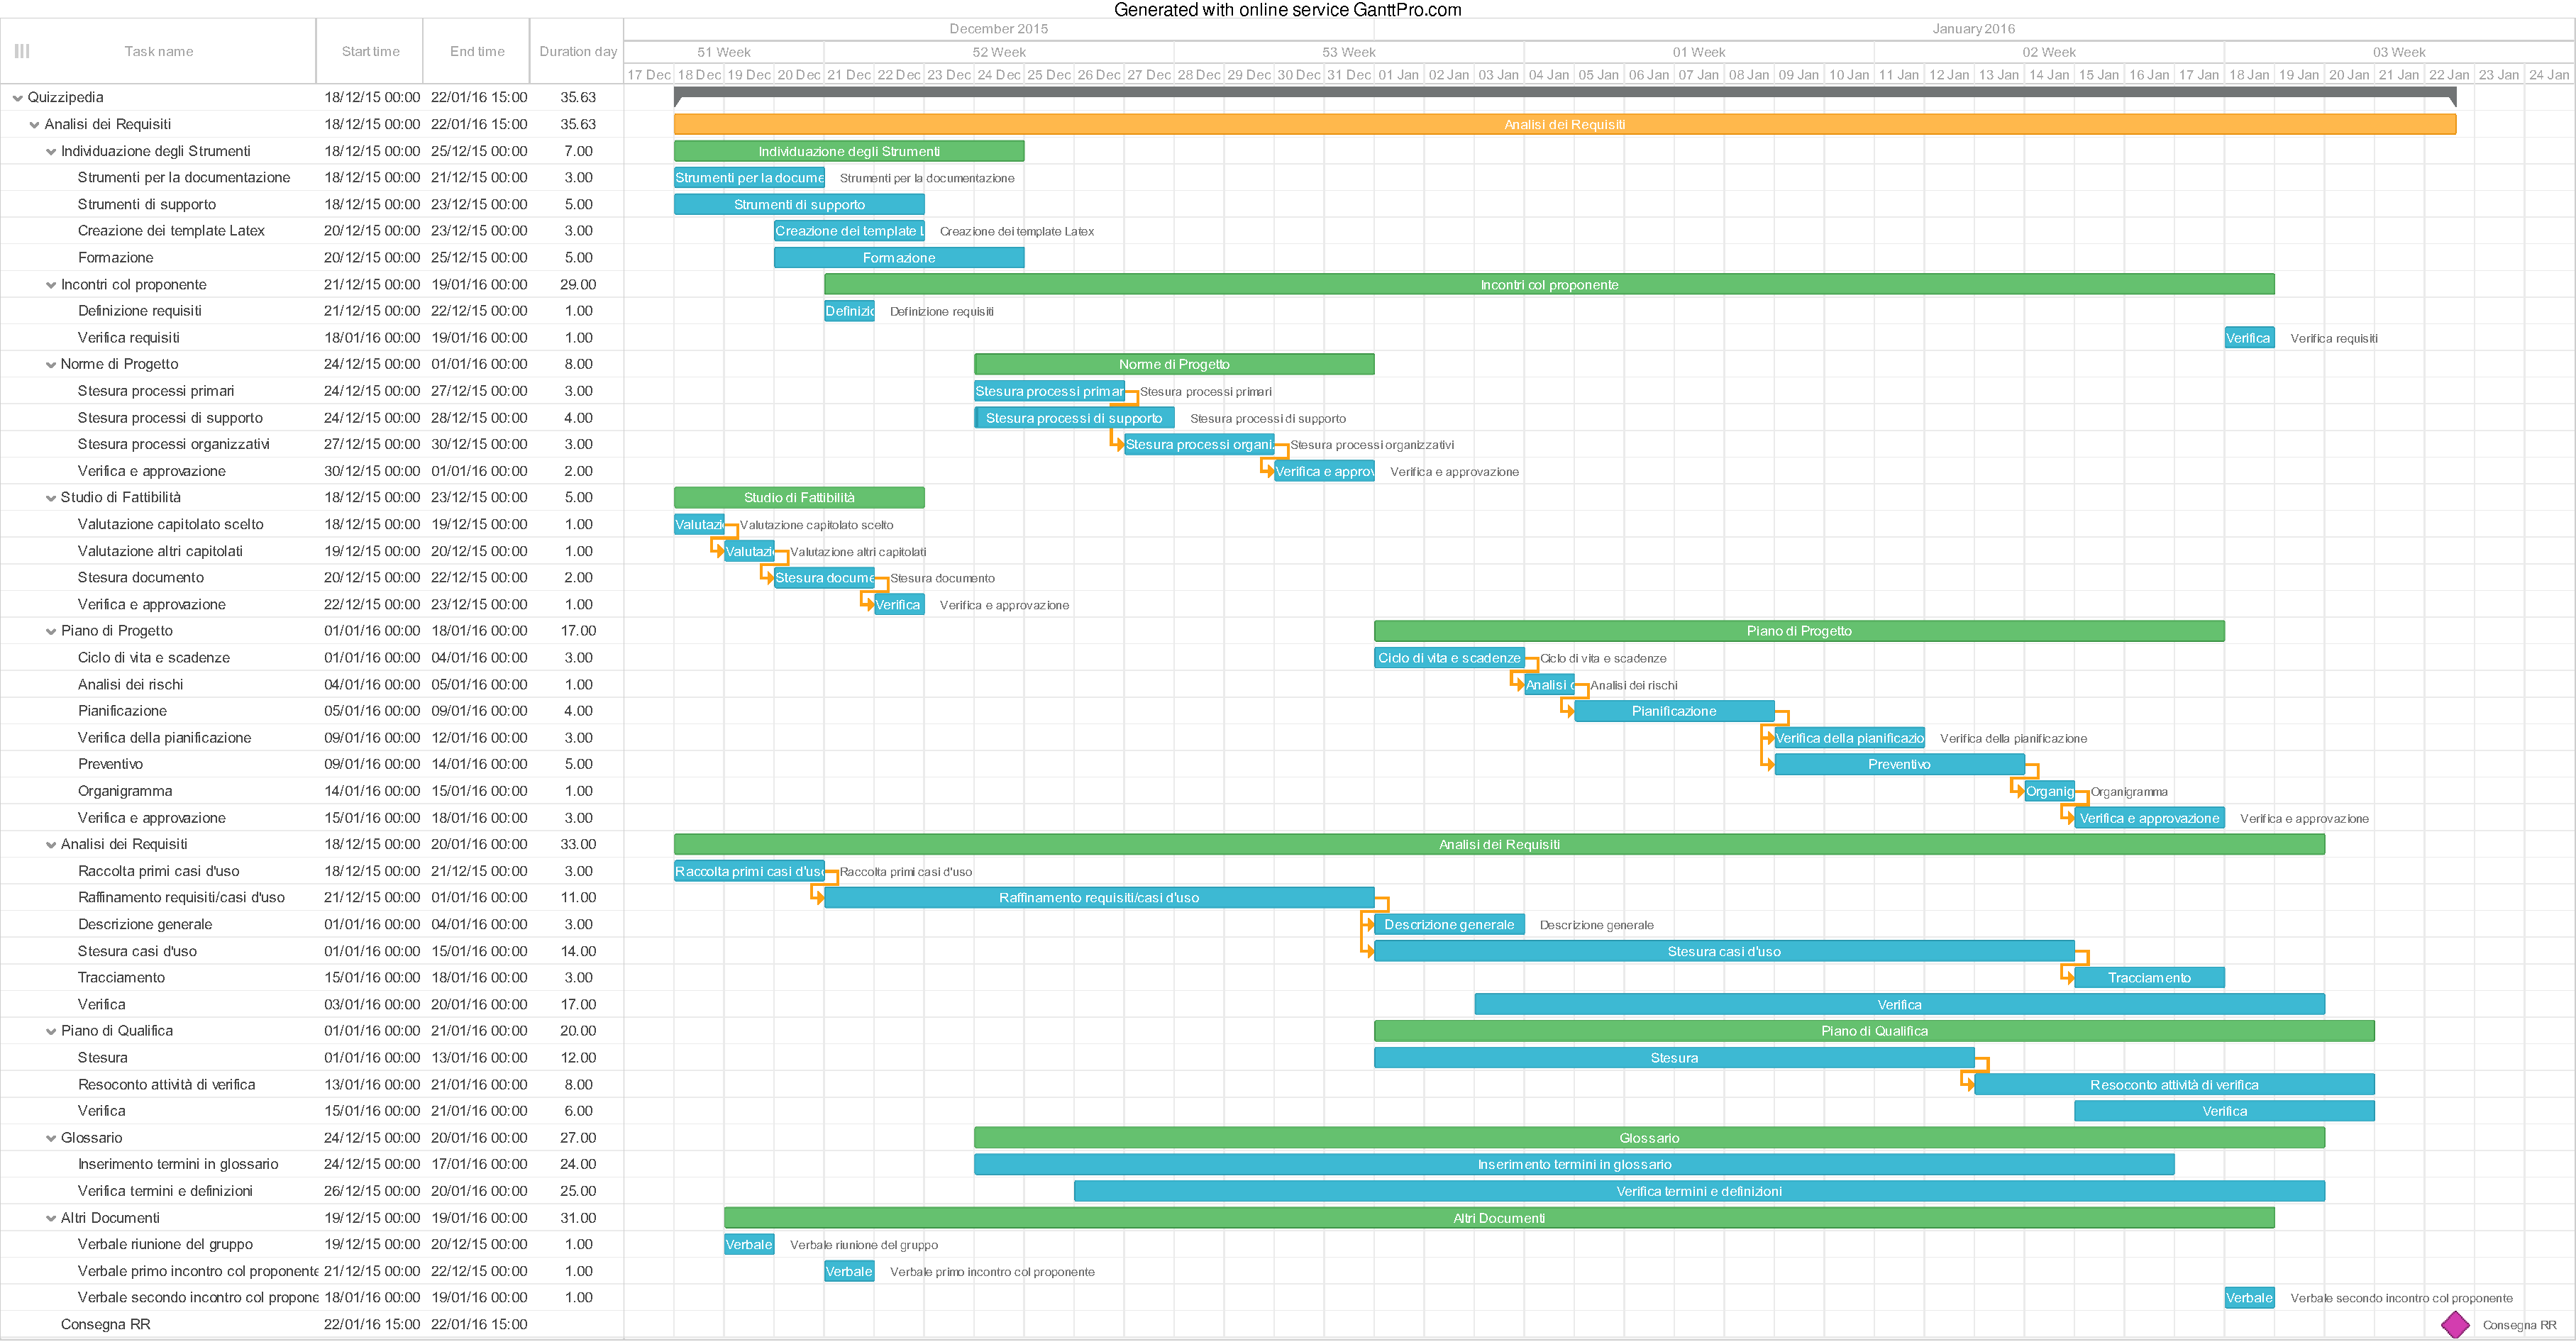
\includegraphics[scale=0.25]{Img/Grafici_Gantt/Analisi_dei_requisiti.pdf}
		\caption{ \gl{Diagramma di Gantt}: Attività di analisi dei requisiti}
	\end{figure}
	
	\subsection{Attività di Raffinamento dei requisiti}
	\subsubsection{Periodo}
	Dal 16.02.2016 al 23.02.2016.\\
	Comincia dopo aver preso visione dell'esito della Revisione dei Requisiti e dura il tempo necessario per una revisione dei documenti.
	
	
	\subsubsection{Sottoattività}
	\begin{itemize}
		\item \bold{Correzione e incremento:} in base all'esito della Revisione dei Requisiti e agli appunti del proponente, vengono corretti e incrementati i documenti precedentemente prodotti. I documenti così approvati passano alla loro v2.0.
	\end{itemize}
	
	%GANTT 2
	\newpage
	\begin{figure}
		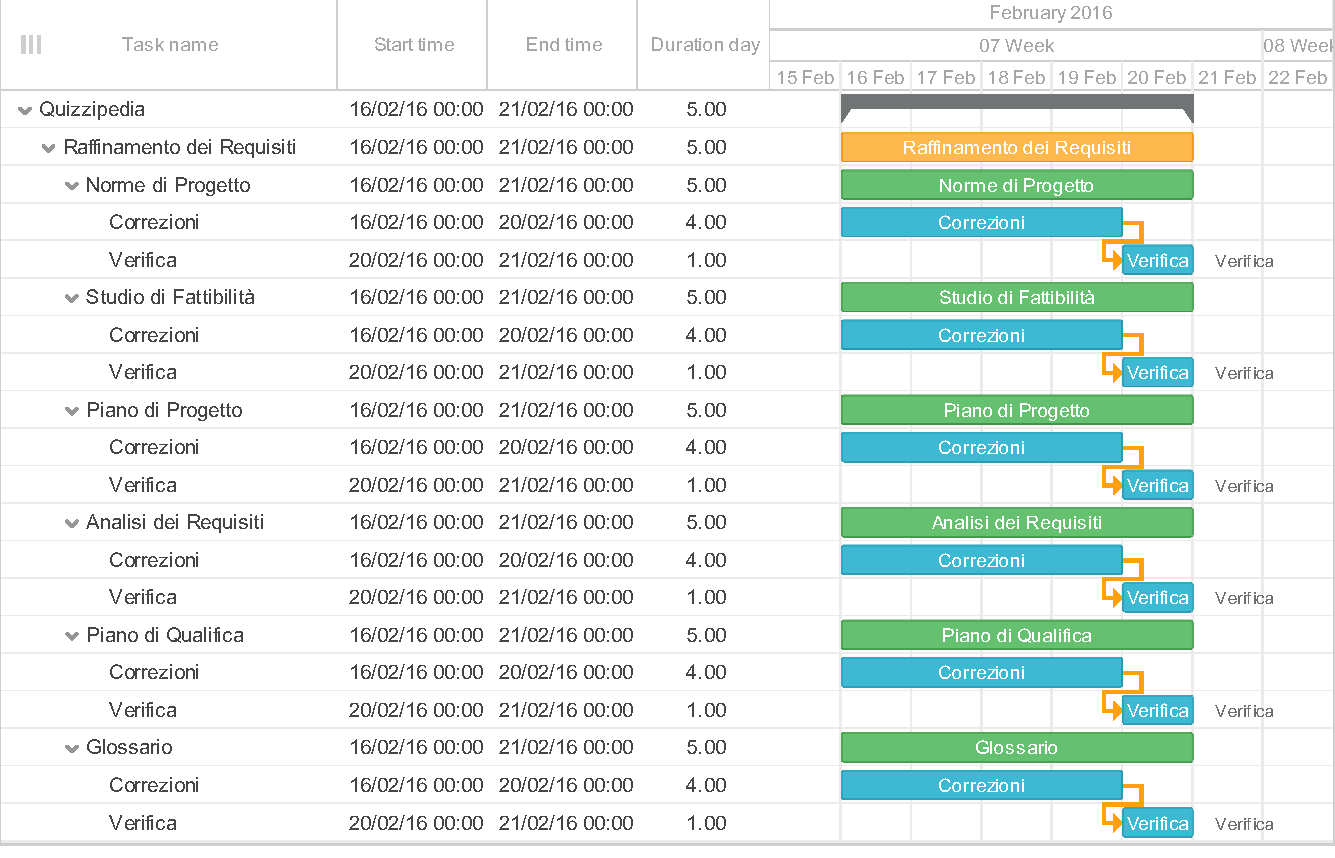
\includegraphics[scale=0.7]{Img/Grafici_Gantt/Raffinamento_requisiti.pdf}
		\caption{ \gl{Diagramma di Gantt}: Raffinamento dei requisiti}
	\end{figure}
	
	\subsection{Attività di Progettazione architetturale}
	\subsubsection{Periodo}
	Dal 24.02.2016 al 11.04.2016.\\
	Segue immediatamente la fine dell'attività di Raffinamento dei requisiti  e termina con un incontro col proponente per illustrargli l'architettura scelta e con la consegna dei documenti per la Revisione di Progettazione.
	
	\subsubsection{Sottattività}
	\begin{itemize}
		\item \bold{Creazione di nuovi documenti:} viene redatto il documento \doc{Specifica Tecnica}. La sua stesura è la sottoattività principale;  vengono fatte scelte progettuali riguardanti il prodotto come, per esempio, i \gl{design pattern}.
		\item \bold{Incremento e verifica dei documenti precedenti:}
		\begin{description}
			\item \bold{Norme di Progetto:} vengono incrementate per poter redigere il documento \doc{Specifica Tecnica v1.0}. Dopo esser stato verificato e approvato il documento è nella sua versione \doc{Norme di Progetto v3.0}.
			\item \bold{Piano di Progetto:} se necessario, viene modificato alla luce del reale avanzamento delle attività;  vengono aggiunti i consuntivi delle attività terminate e il documento viene quindi approvato, passando alla versione \doc{Piano di Progetto v3.0}.
			\item \bold{Analisi dei Requisiti:} come conseguenza della scrittura della \doc{Specifica Tecnica} può subire modifiche; il documento così approvato sarà il \doc{Piano di Progetto v3.0}.
			\item \bold{Piano di Qualifica:} viene aggiornato conseguentemente all'avanzamento del progetto e vengono pianificati i test che il gruppo prevede di svolgere sul proprio prodotto. Si ottiene il documento \doc{Piano di Qualifica v.3.0}.
			\item \bold{Glossario:} vengono costantemente aggiunte le eventuali definizioni emerse durante le sottoattività in corso.  Il documento finale è il \doc{Glossario v3.0}.
		\end{description}	
		\item \bold{Incontro col proponente:} viene fissato un incontro col proponente per illustrargli l'architettura scelta.	 
	\end{itemize}
	
	%GANTT 3
	\begin{figure}[!ht]
		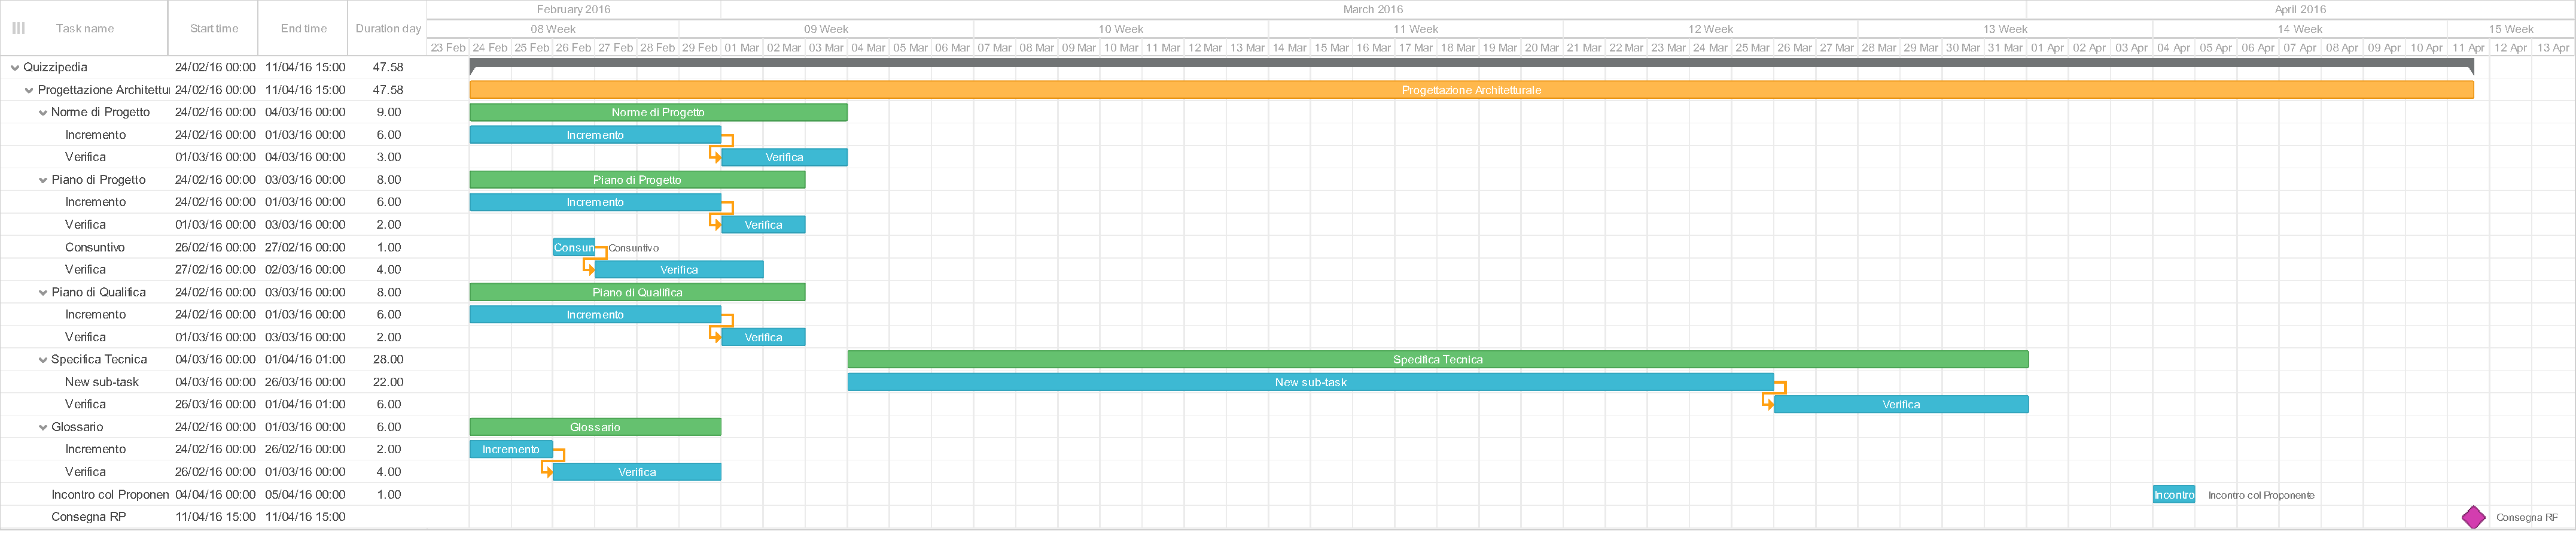
\includegraphics[scale=0.2]{Img/Grafici_Gantt/Progettazione_architetturale.pdf}
		\caption{ \gl{Diagramma di Gantt}: Progettazione architetturale}
	\end{figure}
	
	\subsection{Attività di Progettazione di dettaglio e codifica }
	\subsubsection{Periodo}
	Dal 12.04.2016 al 16.05.2016.\\
	Segue immediatamente l'attività precedente e termina con la consegna della documentazione per accedere alla Revisione di Qualifica.
	
	
	\subsubsection{Sottattività}
	\begin{itemize}
		\item \bold{Incremento e verifica dei documenti precedenti:} se necessario, verranno incrementati o corretti i documenti già scritti in modo simile a quanto già descritto nelle attività precedenti, i documenti così approvati passano alla versione successiva.
		\item \bold{Creazione di nuovi documenti:} vengono redatti i seguenti documenti:
		\begin{description}
			\item \bold{Definizione di Prodotto:} si procede alla stesura di \doc{Definizione di Prodotto v1.0}, che definisce la struttura del prodotto che il gruppo intende sviluppare seguendo le direttive della \doc{Specifica Tecnica}.
			\item \bold{Manuale Utente:} stesura documento \doc{Manuale Utente v1.0}.
			\item \bold{Manuale Sviluppatore:} stesura documento \doc{Manuale Sviluppatore v1.0}.
		\end{description}	
		\item \bold{Codifica:} i \italics{Programmatori} hanno il compito di codificare  requisiti seguendo le direttive della \doc{Definizione di prodotto}.		 
	\end{itemize}
	
	%GANTT 4
	\newpage
	\begin{figure}[!ht]
		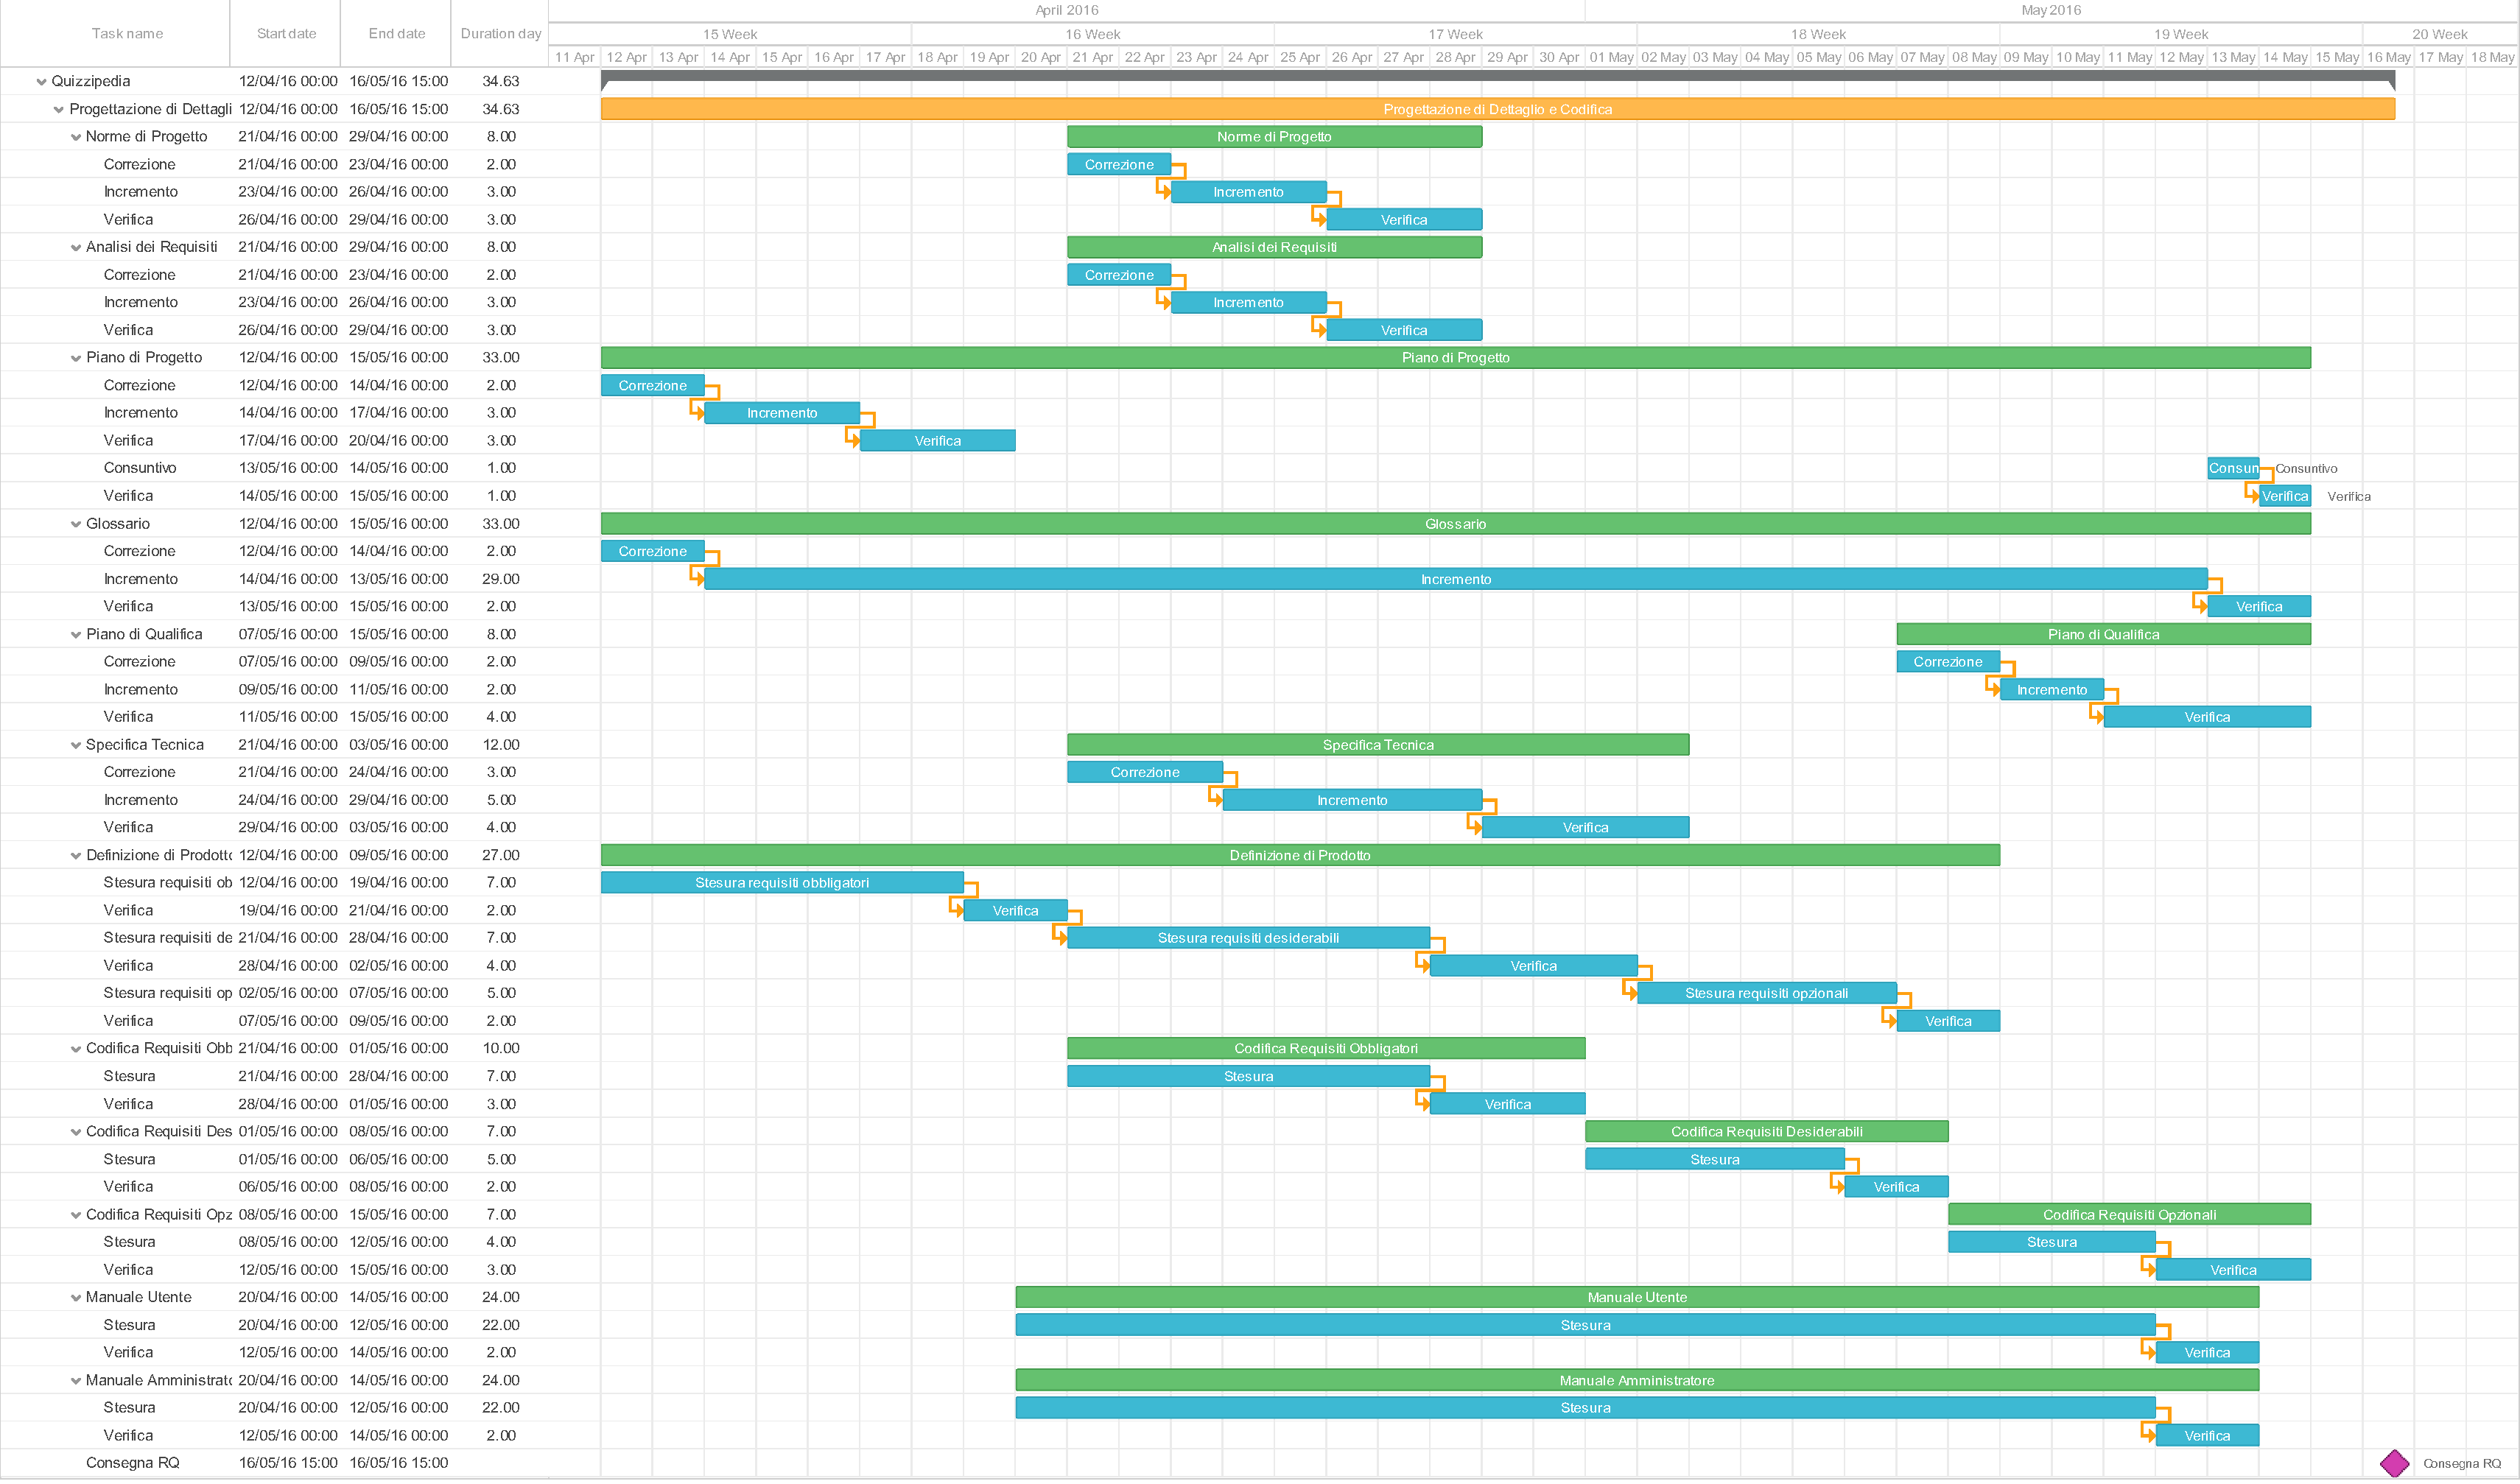
\includegraphics[scale=0.25]{Img/Grafici_Gantt/Progettazione(dett-cod).pdf}
		\caption{ \gl{Diagramma di Gantt}: Progettazione di dettaglio e codifica}
	\end{figure}
	
	\subsection{Attività di validazione}
	\subsubsection{Periodo}
	Dal 17.05.2016 al 10.06.2016\\
	Segue immediatamente le attività di progettazione di dettaglio  e termina con la consegna dei documenti necessari per la Revisione di Accettazione.
	
	\subsubsection{Sottattività}
	\begin{itemize}
		\item \bold{Incremento e verifica dei documenti precedenti:} se necessario, verranno incrementati o corretti i documenti già scritti in modo simile a quanto già descritto nelle attività precedenti, i documenti così approvati passano alla versione successiva.
		\item \bold{Esecuzione di test:} esecuzione di test di validazione come descritto nel \doc{Piano di Qualifica}, che verrà conseguentemente aggiornato.
		\item \bold{Individuazione e correzione di bug.} 
		\item \bold{Collaudo del prodotto finale prima della consegna.} 
	\end{itemize}
	
	%GANTT 5
	\newpage
	\begin{figure}[!ht]
		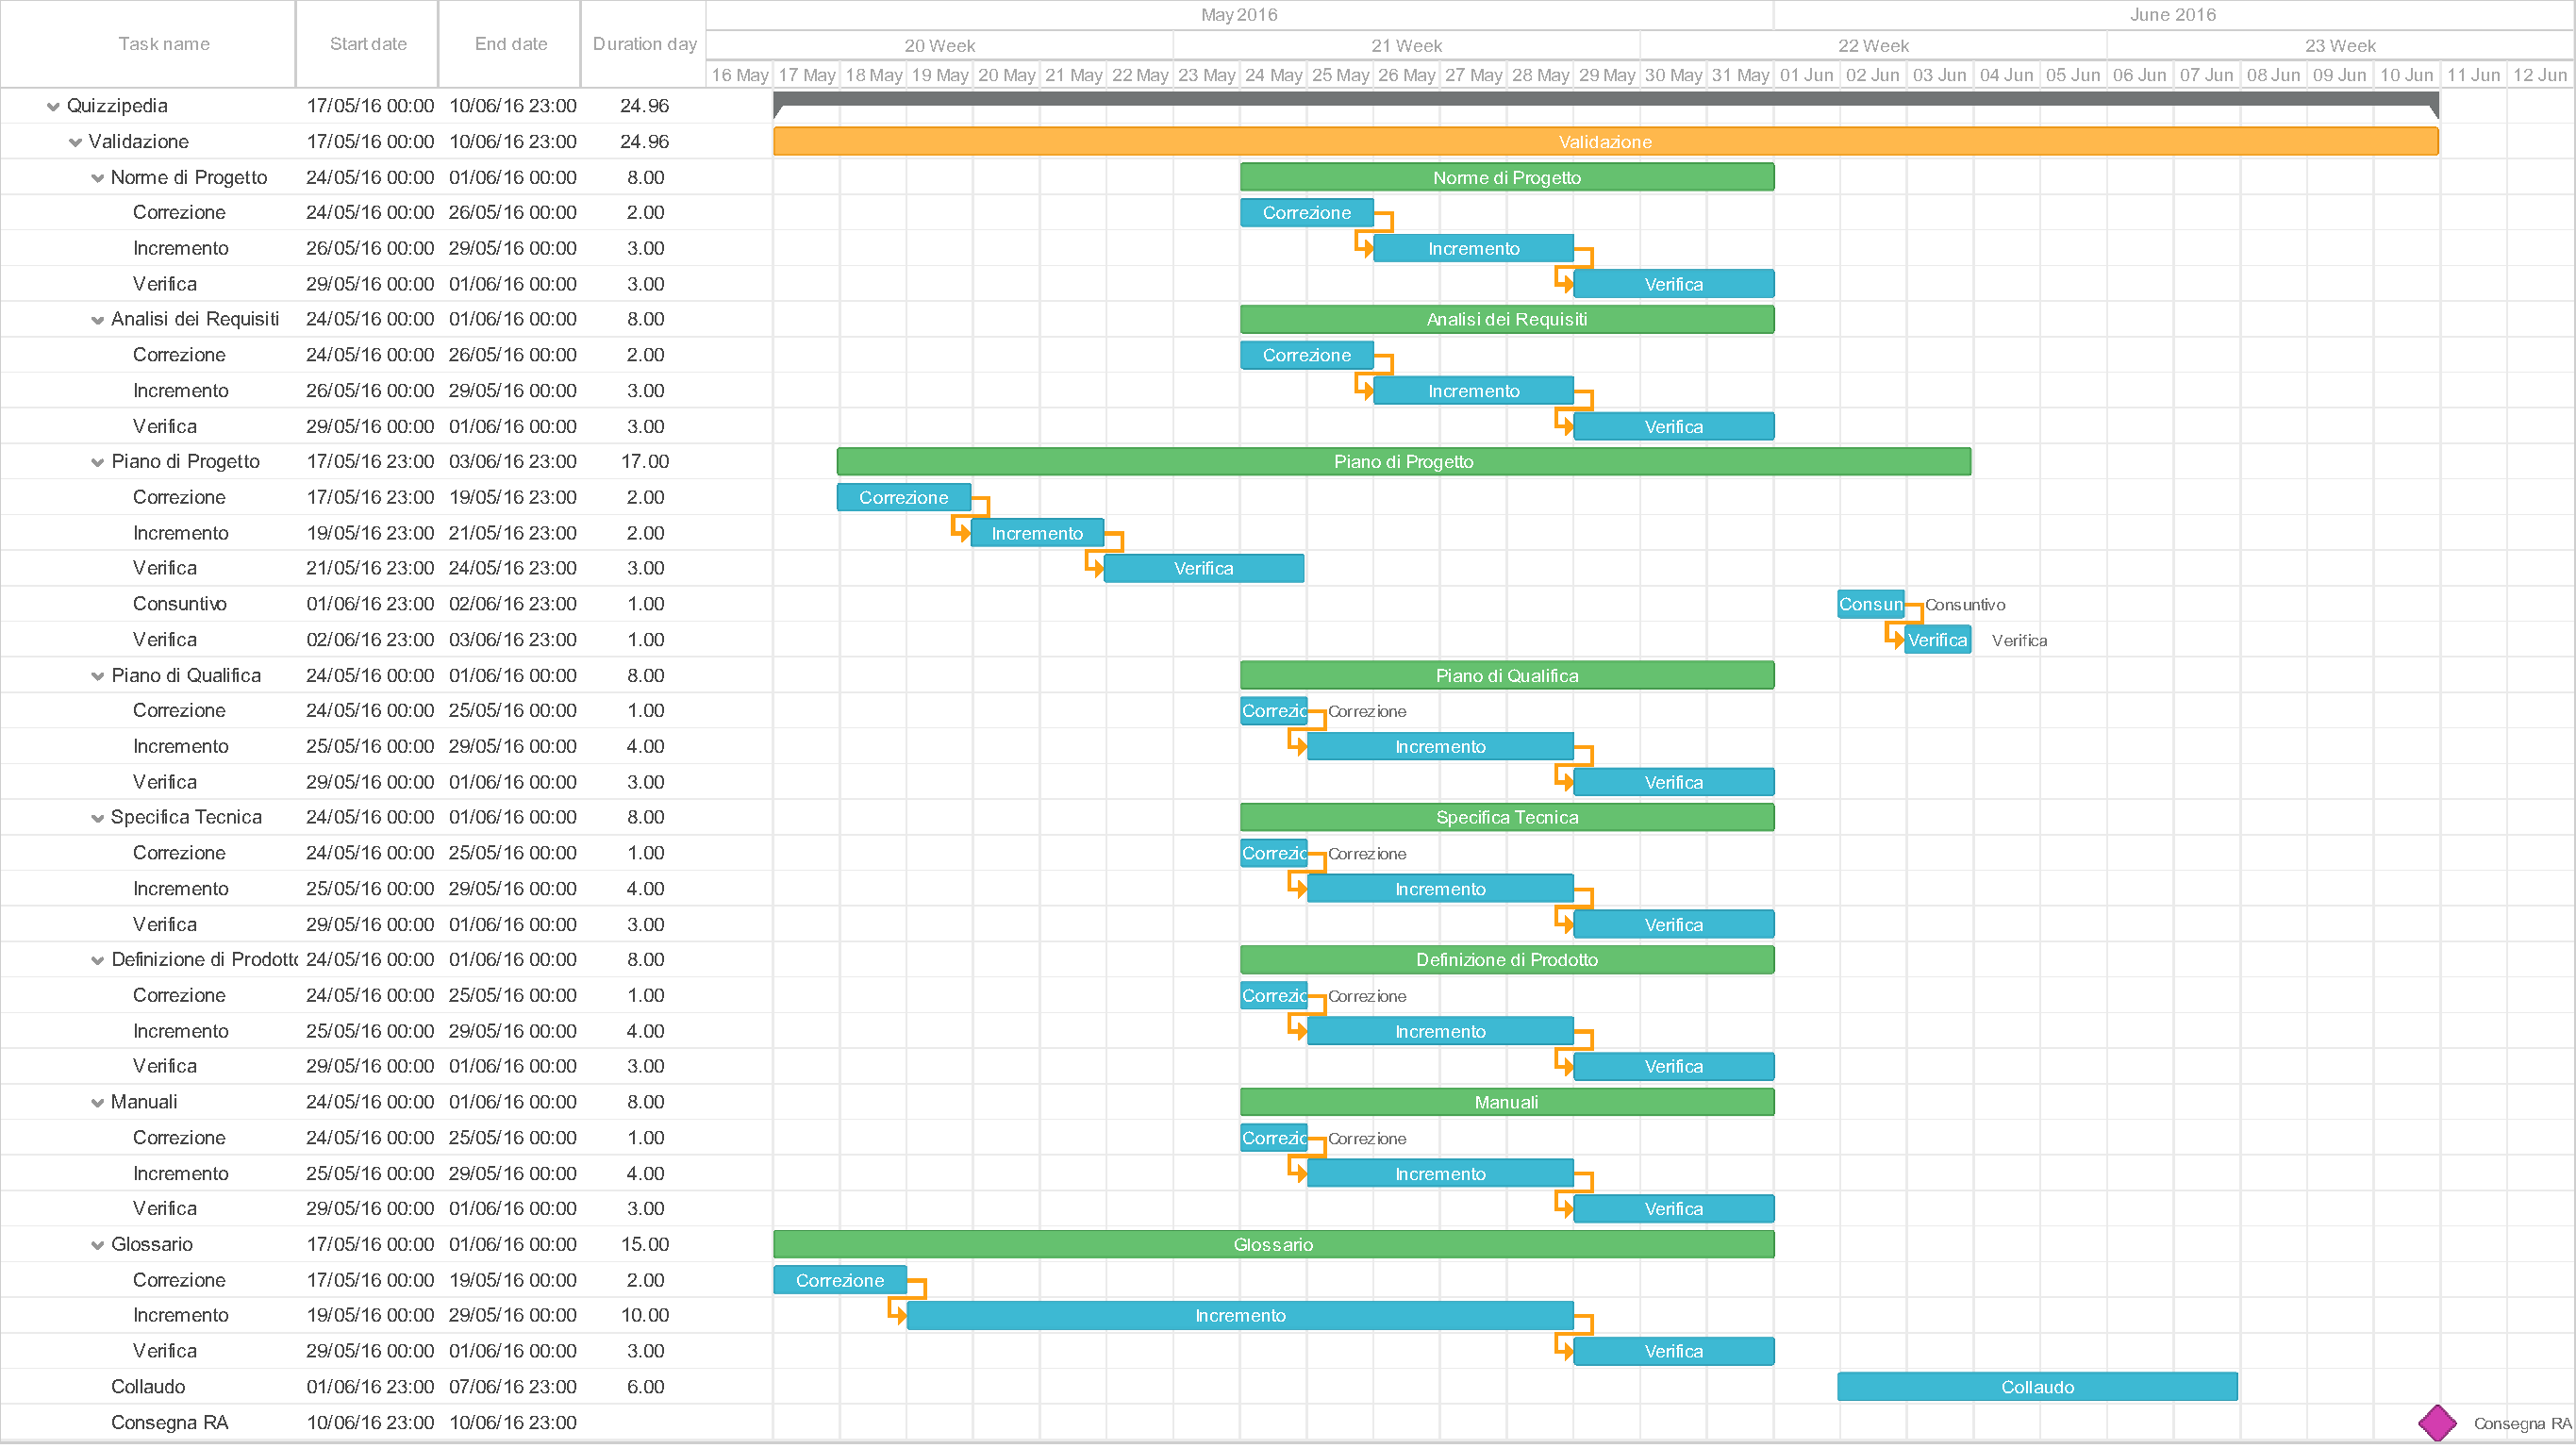
\includegraphics[scale=0.3]{Img/Grafici_Gantt/Validazione.pdf}
		\caption{ \gl{Diagramma di Gantt}: Validazione}
	\end{figure}
	
	\newpage
	\section {Preventivo}\label{Preventivo}
	Segue il preventivo per le fasi a carico del committente. È possibile prendere visione delle ore di investimento nell'\hyperref[Investimento]{Appendice B}.
	
	\subsection{Attività di progettazione architetturale}
	\subsubsection{Prospetto orario}
	Durante questa attività ogni componente del gruppo ricoprirà i seguenti ruoli:
	
	\begin{tabella}{l!{\VRule}c!{\VRule}c!{\VRule}c!{\VRule}c!{\VRule}c!{\VRule}c!{\VRule}c!{\VRule}c}
		
		\color{white} \bold{Nome} & \color{white} \bold{Responsabile} &\color{white} \bold{Amm} & \color{white} \bold{An} & \color{white} \bold{Pt} & \color{white} \bold{Pr} & \color{white} \bold{Ver} & \color{white} \bold{Ore totali persona} \\
		\endfirsthead
		Giacomo Beltrame & 0 & 0 & 5 & 20 & 0 & 0 & 25\\
		Rudy Berton & 0 & 10 & 0 & 0 & 0 & 13 & 23\\
		Simone Boccato & 0 & 0 & 0 & 5 & 0 & 20 & 25\\
		Michela De Bortoli & 10 & 0 & 0 & 15 & 0 & 0 & 25\\
		Vassilikì Menarin & 0 & 0 & 0 & 15 & 0 & 12 & 27\\
		Filippo Tesser & 10 & 0 & 8 & 0 & 0 & 8 & 26\\
		Miki Violetto & 0 & 7 & 0 & 10 & 0 & 6 & 23\\   
		
		\rowcolor{white}  
		\caption{Prospetto orario attività di progettazione architetturale}	    	
		
	\end{tabella}
	
	\begin{figure}[!ht]
		\centering
		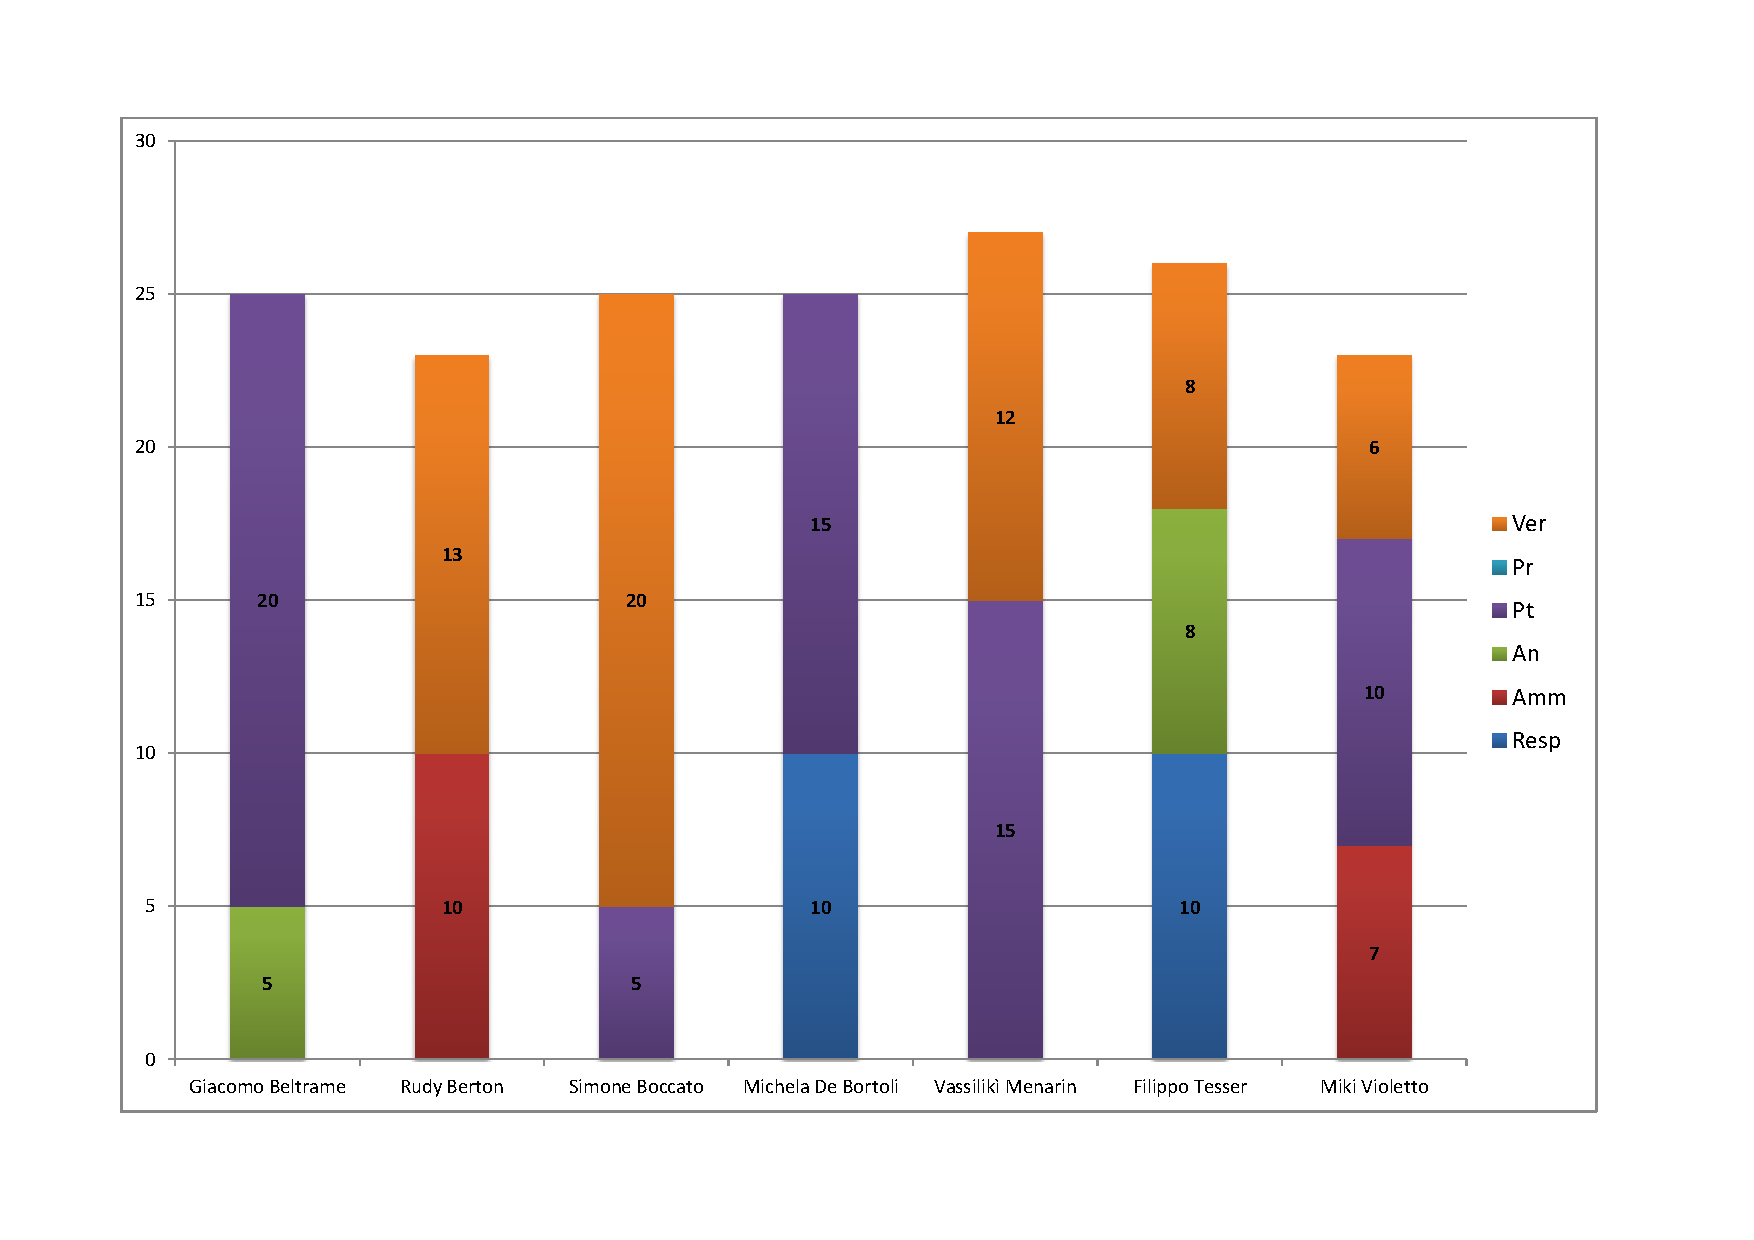
\includegraphics[scale=0.5]{Img/Grafici/Ist03.pdf}
		\caption{ Istogramma: Prospetto orario attività di progettazione architetturale}
	\end{figure}
	
	\newpage
	\subsubsection{Prospetto economico}
	Il prospetto economico per questa attività è illustrato in tabella. 
	
	\begin{tabella}{l!{\VRule}c!{\VRule}c}
		
		\color{white} \bold{Ruolo} & \color{white} \bold{Ore} &\color{white} \bold{Spese} \\
		\endfirsthead
		Responsabile & 20 & € 600 \\
		Amministratore & 17 & € 340\\
		Analista & 13 & € 325 \\
		Progettista & 65 & € 1430 \\
		Programmatore & 0 & € 0 \\
		Verificatore & 59 & € 885 \\
		Totale & 174 & € 3580\\
		
		\rowcolor{white}  
		\caption{Prospetto economico attività di progettazione architetturale}	    	
		
	\end{tabella}
	
	\begin{figure}[!ht]
		\centering
		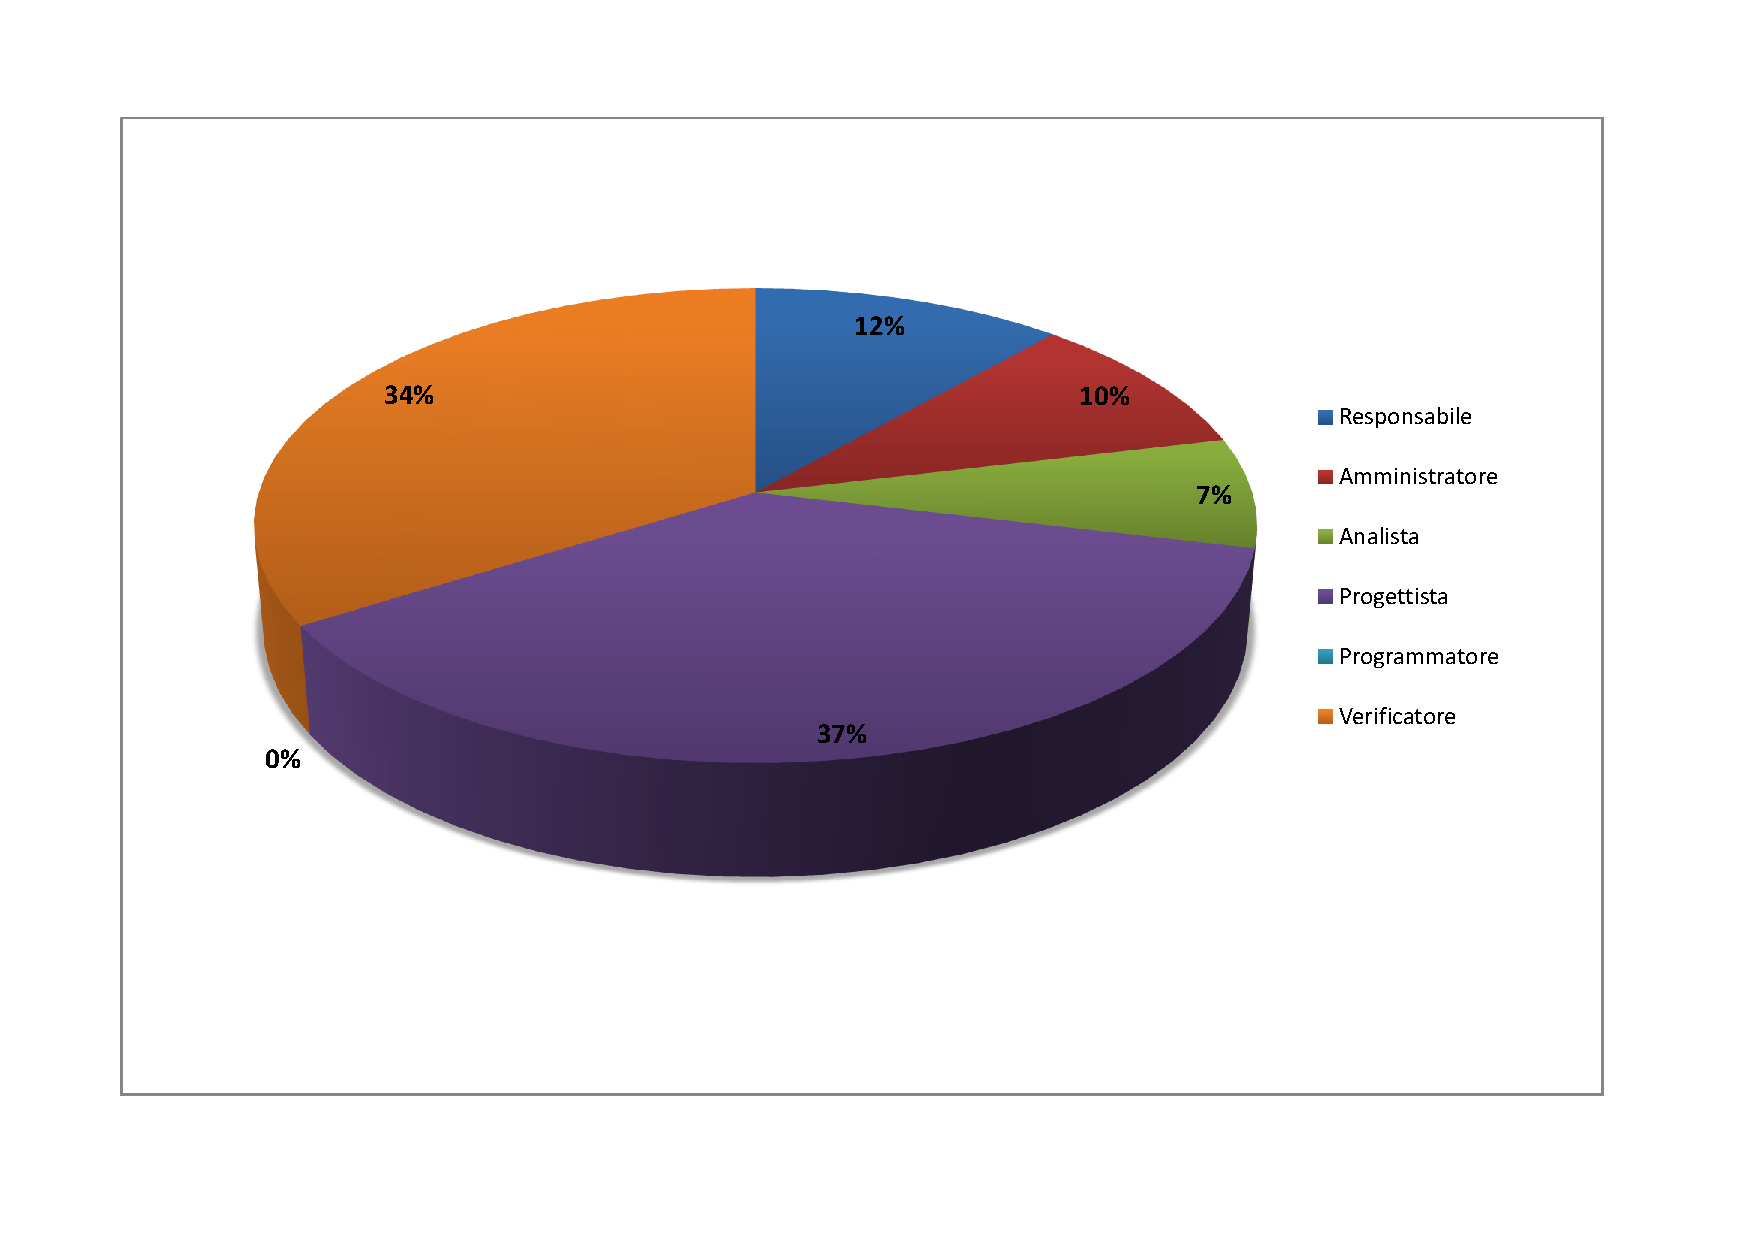
\includegraphics[scale=0.5]{Img/Grafici/Aer03.pdf}
		\caption{ Areogramma: Ore per ruolo durante l'attività di progettazione architetturale}
	\end{figure}
	
	\newpage
	\subsection{Attività di progettazione di dettaglio e codifica}
	\subsubsection{Prospetto orario}
	Durante questa attività ogni componente del gruppo ricoprirà i seguenti ruoli:
	
	\begin{tabella}{l!{\VRule}c!{\VRule}c!{\VRule}c!{\VRule}c!{\VRule}c!{\VRule}c!{\VRule}c!{\VRule}c}
		
		\color{white} \bold{Nome} & \color{white} \bold{Responsabile} &\color{white} \bold{Amm} & \color{white} \bold{An} & \color{white} \bold{Pt} & \color{white} \bold{Pr} & \color{white} \bold{Ver} & \color{white} \bold{Ore totali persona} \\
		\endfirsthead
		Giacomo Beltrame & 13 & 0 & 6 & 0 & 20 & 18 & 57\\
		Rudy Berton & 0 & 0 & 0 & 30 & 0 & 22 & 52\\
		Simone Boccato & 0 & 6 & 0 & 17 & 25 & 7 & 55\\
		Michela De Bortoli & 0 & 10 & 0 & 20 & 25 & 0 & 55\\
		Vassilikì Menarin & 0 & 0 & 7 & 0 & 26 & 21 & 54\\
		Filippo Tesser & 0 & 0 & 0 & 20 & 15 & 16 & 51\\
		Miki Violetto & 0 & 0 & 0 & 12 & 29 & 13 & 54\\   
		
		\rowcolor{white}  
		\caption{Prospetto orario attività di progettazione di dettaglio e codifica}	    	
		
	\end{tabella}
	
	\begin{figure}[!ht]
		\centering
		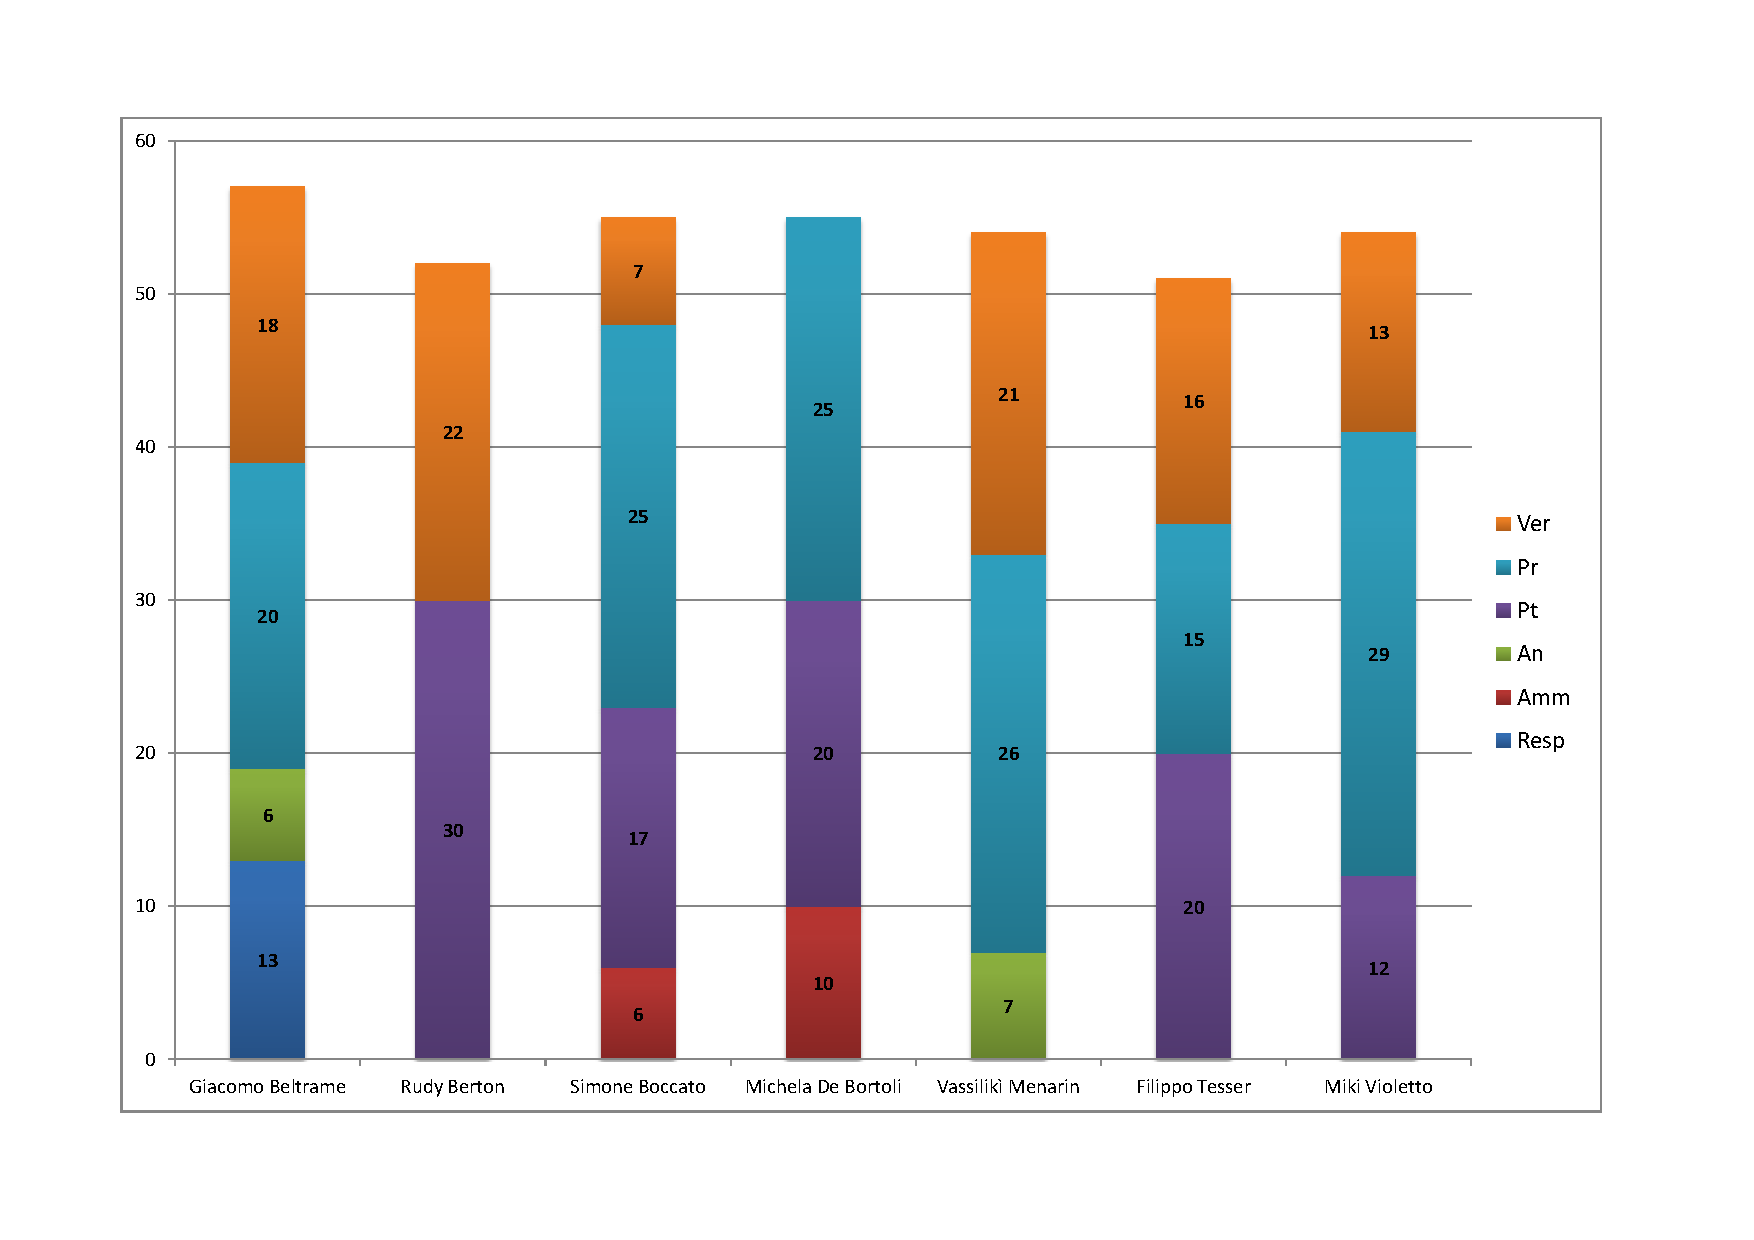
\includegraphics[scale=0.5]{Img/Grafici/Ist04.pdf}
		\caption{ Istogramma: Prospetto orario attività di progettazione di dettaglio e codifica}
	\end{figure}
	
	\newpage
	\subsubsection{Prospetto economico}
	Il prospetto economico per questa attività è illustrato in tabella. 
	
	\begin{tabella}{l!{\VRule}c!{\VRule}c}
		
		\color{white} \bold{Ruolo} & \color{white} \bold{Ore} &\color{white} \bold{Spese} \\
		\endfirsthead
		Responsabile & 13 & € 390 \\
		Amministratore & 16 & € 320\\
		Analista & 13 & € 325 \\
		Progettista & 99 & € 2178 \\
		Programmatore & 140 & € 2100 \\
		Verificatore & 97 & € 1455\\
		Totale & 378 & € 6768\\
		
		\rowcolor{white}  
		\caption{Prospetto economico attività di progettazione di dettaglio e codifica}	    	
		
	\end{tabella}
	
	\begin{figure}[!ht]
		\centering
		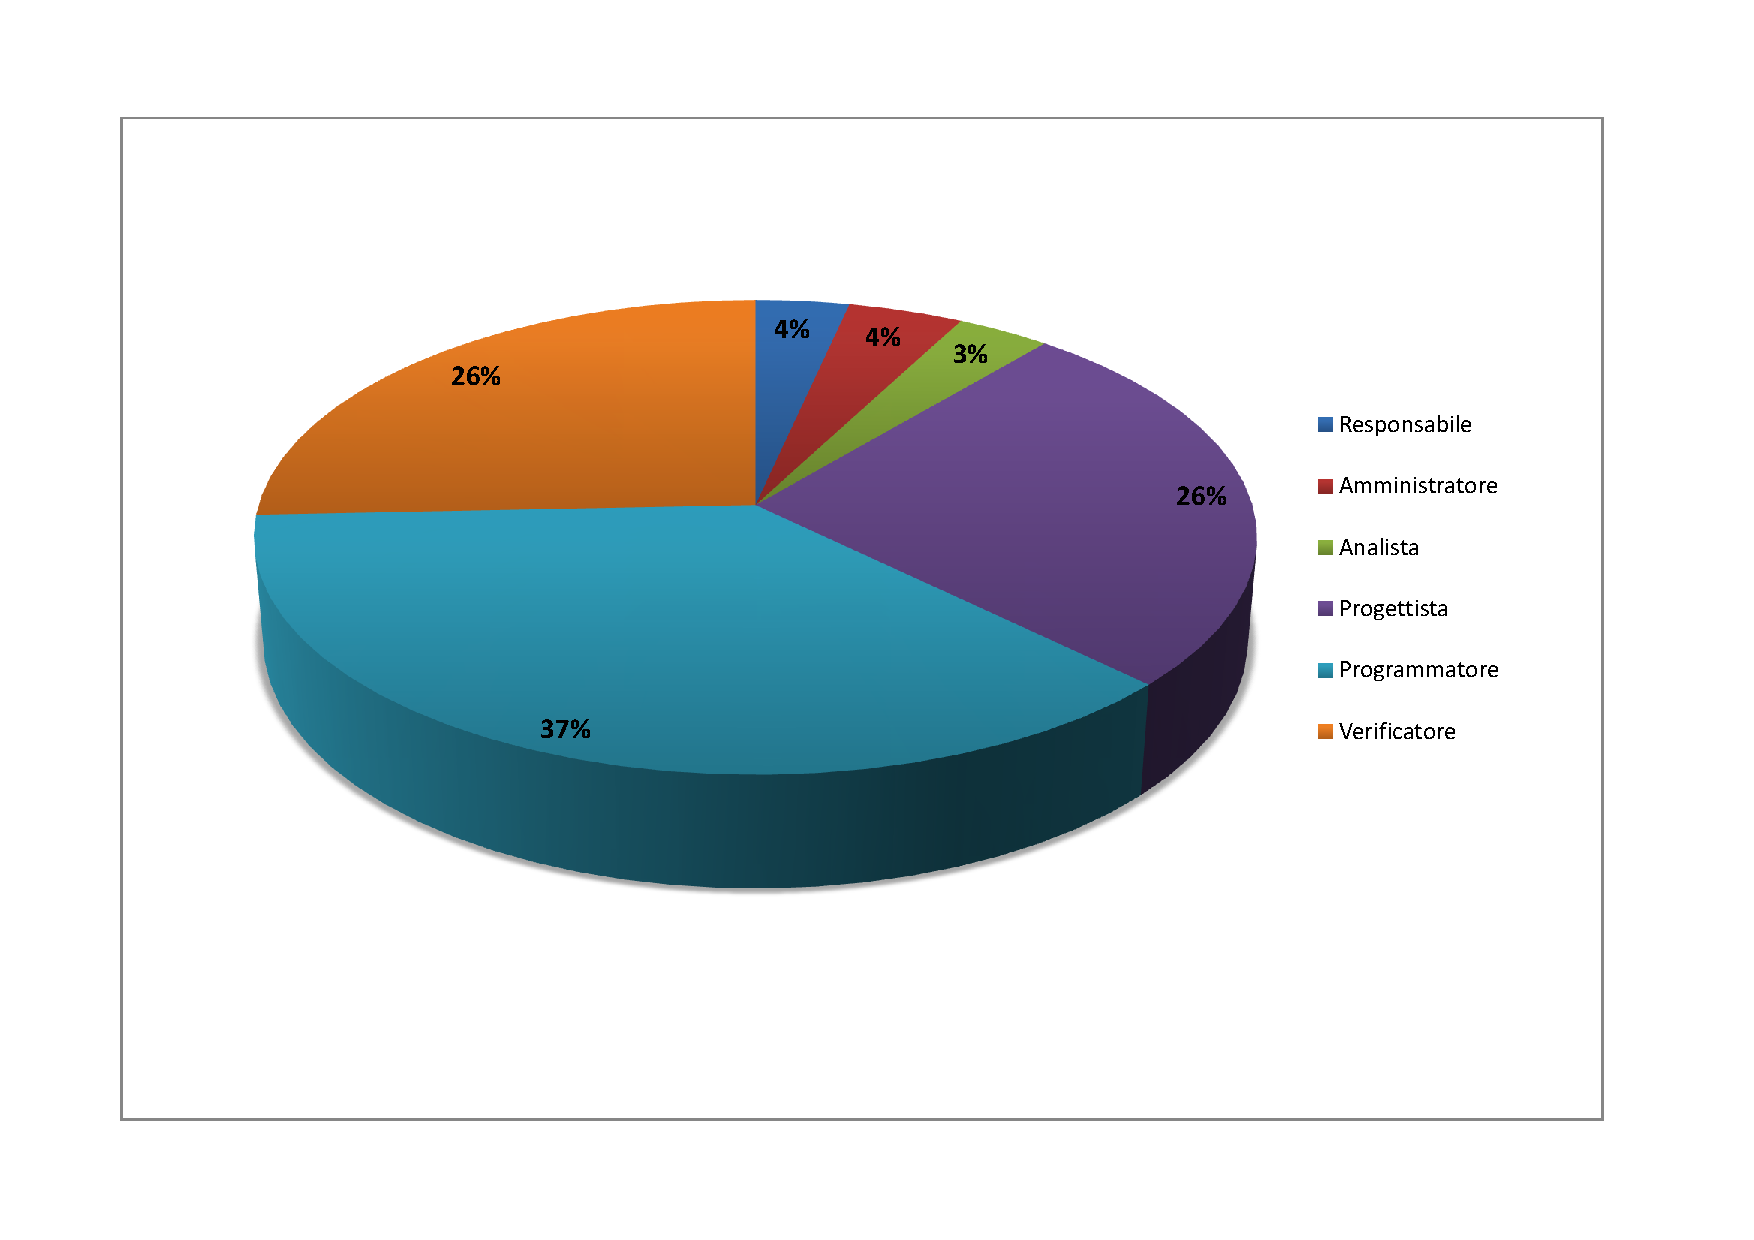
\includegraphics[scale=0.5]{Img/Grafici/Aer04.pdf}
		\caption{ Areogramma: Ore per ruolo durante l'attività di progettazione di dettaglio e codifica}
	\end{figure}
	
	\newpage
	\subsection{Attività di validazione}
	\subsubsection{Prospetto orario}
	Durante questa attività ogni componente del gruppo ricoprirà i seguenti ruoli:
	
	\begin{tabella}{l!{\VRule}c!{\VRule}c!{\VRule}c!{\VRule}c!{\VRule}c!{\VRule}c!{\VRule}c!{\VRule}c}
		
		\color{white} \bold{Nome} & \color{white} \bold{Responsabile} &\color{white} \bold{Amm} & \color{white} \bold{An} & \color{white} \bold{Pt} & \color{white} \bold{Pr} & \color{white} \bold{Ver} & \color{white} \bold{Ore totali persona} \\
		\endfirsthead
		Giacomo Beltrame & 0 & 0 & 0 & 13 & 0 & 7 & 20\\
		Rudy Berton & 15 & 0 & 0 & 0 & 13 & 0 & 28\\
		Simone Boccato & 10 & 0 & 0 & 0 & 0 & 11 & 21\\
		Michela De Bortoli & 0 & 0 & 0 & 10 & 0 & 12 & 22\\
		Vassilikì Menarin & 0 & 11 & 0 & 10 & 0 & 0 & 21\\
		Filippo Tesser & 0 & 0 & 0 & 0 & 10 & 14 & 24\\
		Miki Violetto & 0 & 0 & 0 & 12 & 0 & 12 & 24\\   
		
		\rowcolor{white}  
		\caption{Prospetto orario attività di validazione}	    	
		
	\end{tabella}
	
	\begin{figure}[!ht]
		\centering
		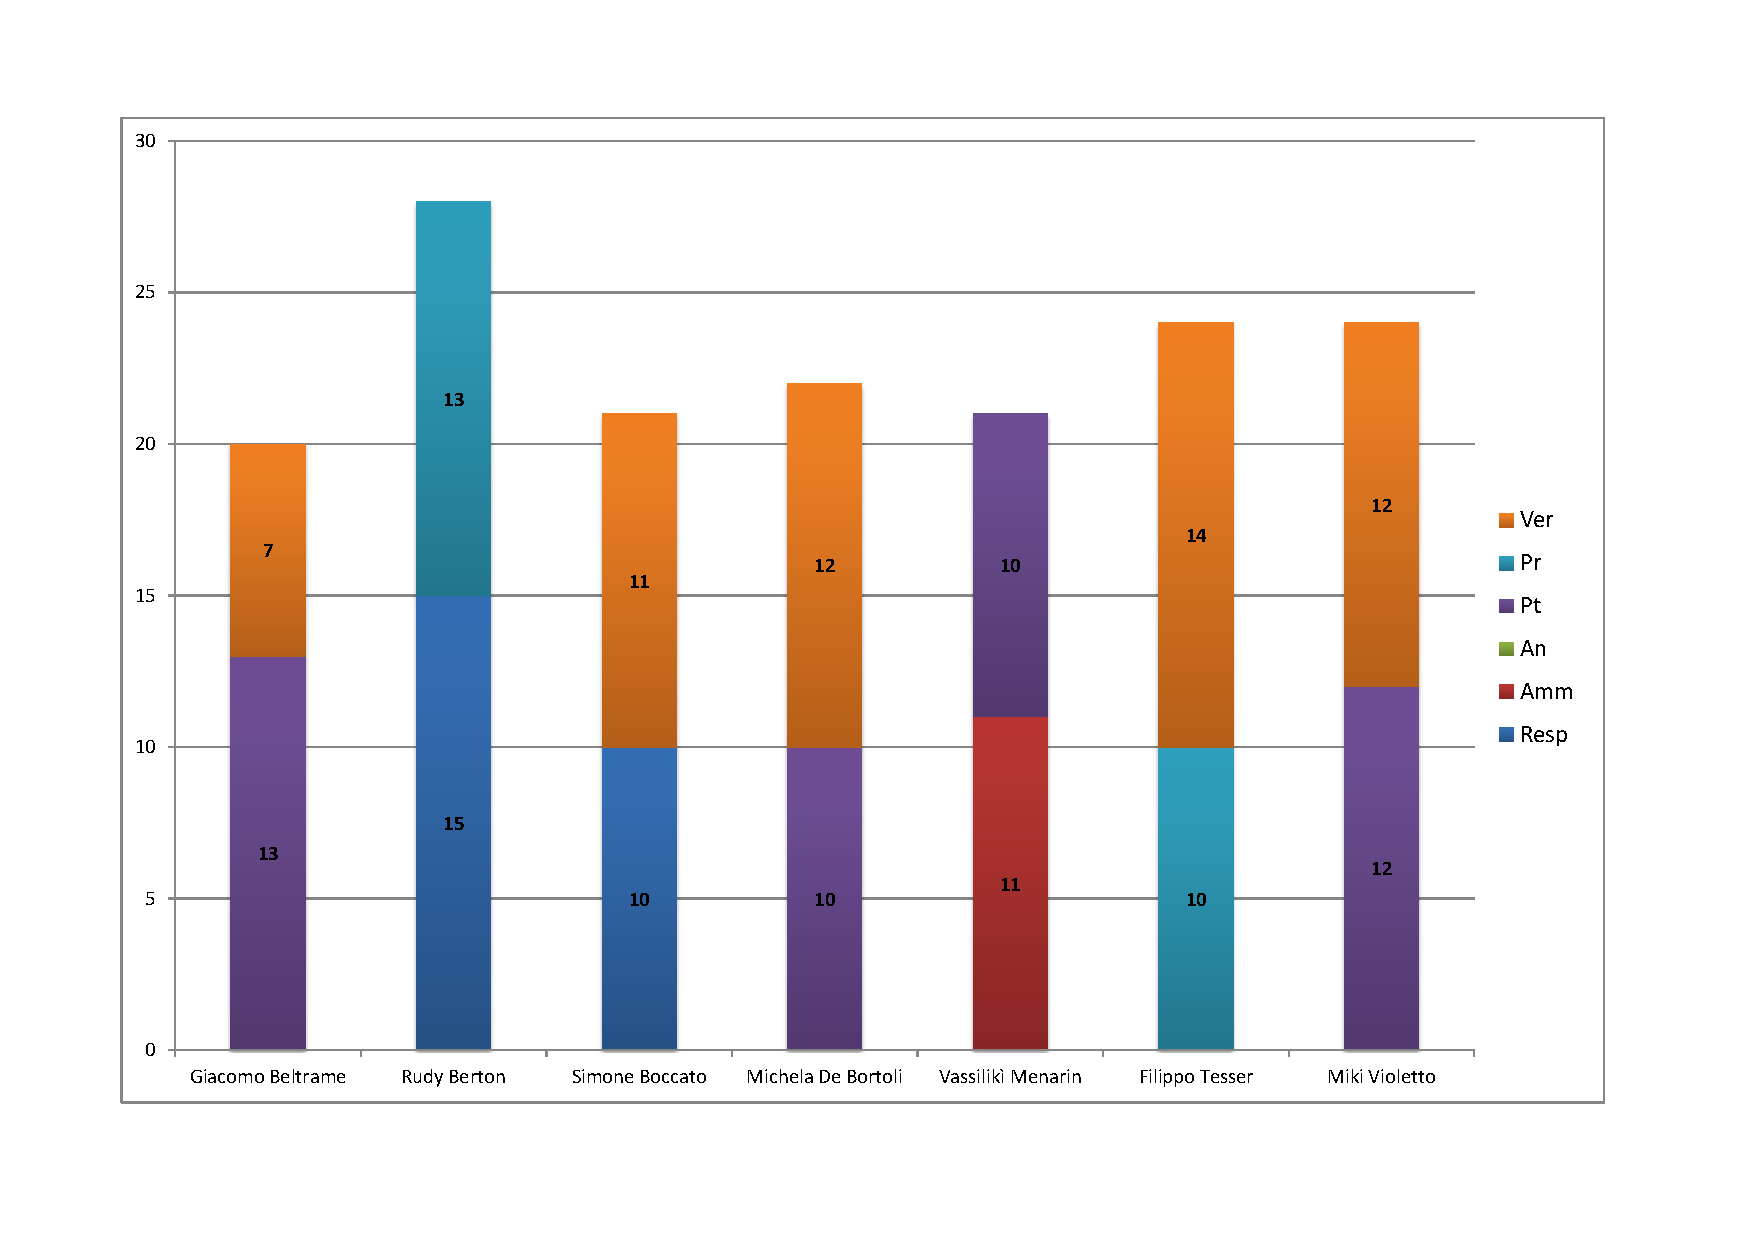
\includegraphics[scale=0.5]{Img/Grafici/Ist05.pdf}
		\caption{ Istogramma: Prospetto orario attività di validazione}
	\end{figure}
	
	\newpage
	\subsubsection{Prospetto economico}
	Il prospetto economico per questa attività è illustrato in tabella. 
	
	\begin{tabella}{l!{\VRule}c!{\VRule}c}
		
		\color{white} \bold{Ruolo} & \color{white} \bold{Ore} &\color{white} \bold{Spese} \\
		\endfirsthead
		Responsabile & 25 & € 750 \\
		Amministratore & 11 & € 220\\
		Analista & 0 & € 0 \\
		Progettista & 45 & € 990 \\
		Programmatore & 23 & € 345 \\
		Verificatore & 56 & € 840\\
		Totale & 160 & € 3145\\
		
		\rowcolor{white}  
		\caption{Prospetto economico attività di validazione}	    	
		
	\end{tabella}
	
	\begin{figure}[!ht]
		\centering
		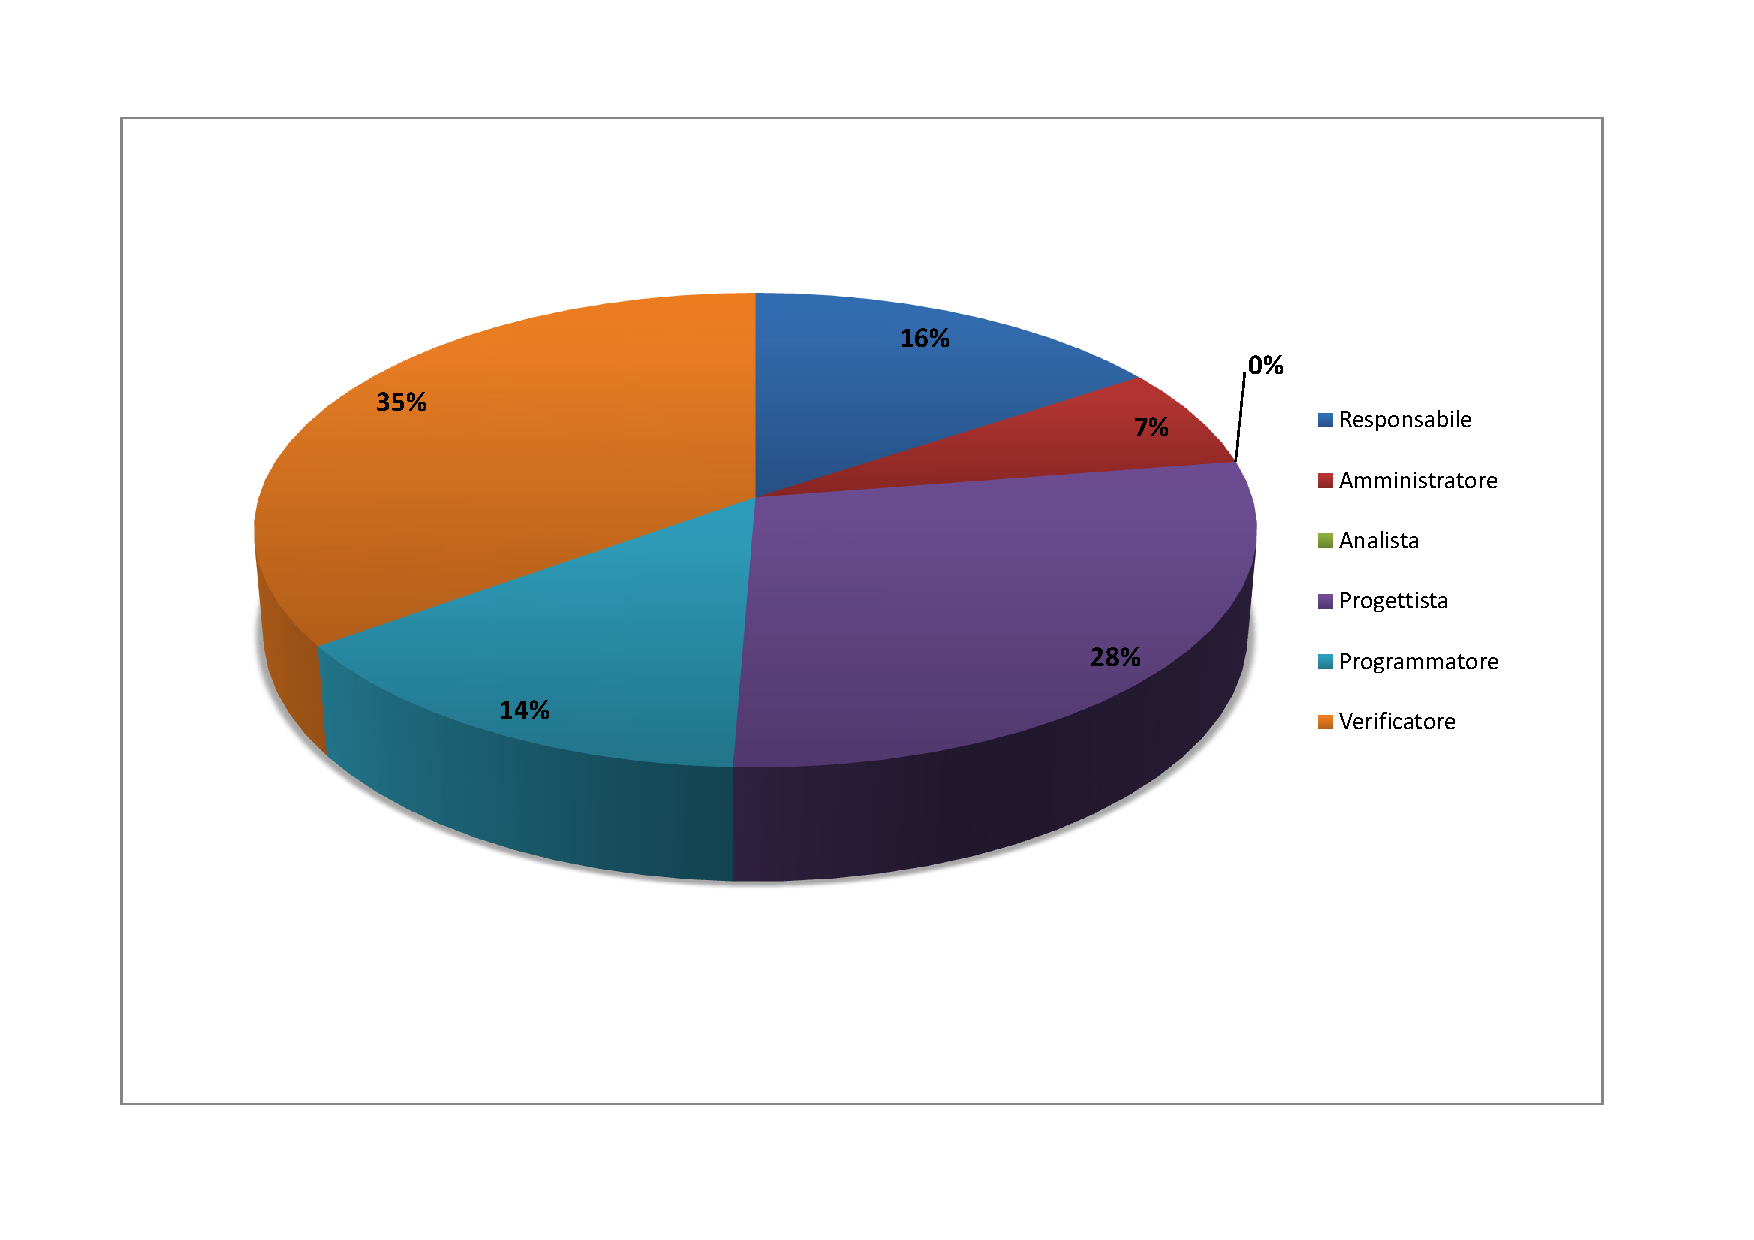
\includegraphics[scale=0.5]{Img/Grafici/Aer05.pdf}
		\caption{ Areogramma: Ore per ruolo durante l'attività di validazione}
	\end{figure}
	
	\newpage
	\subsection{Totale}
	\subsubsection{Prospetto orario}
	In tabella sono riassunte le ore totali rendicontate per ruolo che ogni membro del gruppo ricoprirà:
	
	\begin{tabella}{l!{\VRule}c!{\VRule}c!{\VRule}c!{\VRule}c!{\VRule}c!{\VRule}c!{\VRule}c!{\VRule}c}
		
		\color{white} \bold{Nome} & \color{white} \bold{Responsabile} &\color{white} \bold{Amm} & \color{white} \bold{An} & \color{white} \bold{Pt} & \color{white} \bold{Pr} & \color{white} \bold{Ver} & \color{white} \bold{Ore totali persona} \\
		\endfirsthead
		Giacomo Beltrame & 13 & 0 & 11 & 33 & 20 & 25 & 102\\
		Rudy Berton & 15 & 10 & 0 & 30 & 13 & 35 & 103\\
		Simone Boccato & 10 & 6 & 0 & 22 & 25 & 38 & 101\\
		Michela De Bortoli & 10 & 10 & 0 & 45 & 25 & 12 & 102\\
		Vassilikì Menarin & 0 & 11 & 7 & 25 & 26 & 33 & 102\\
		Filippo Tesser & 10 & 0 & 8 & 20 & 25 & 38 & 101\\
		Miki Violetto & 0 & 7 & 0 & 34 & 29 & 31 & 101\\   
		
		\rowcolor{white}  
		\caption{Prospetto orario rendicontato totale}	    	
		
	\end{tabella}
	
	\begin{figure}[!ht]
		\centering
		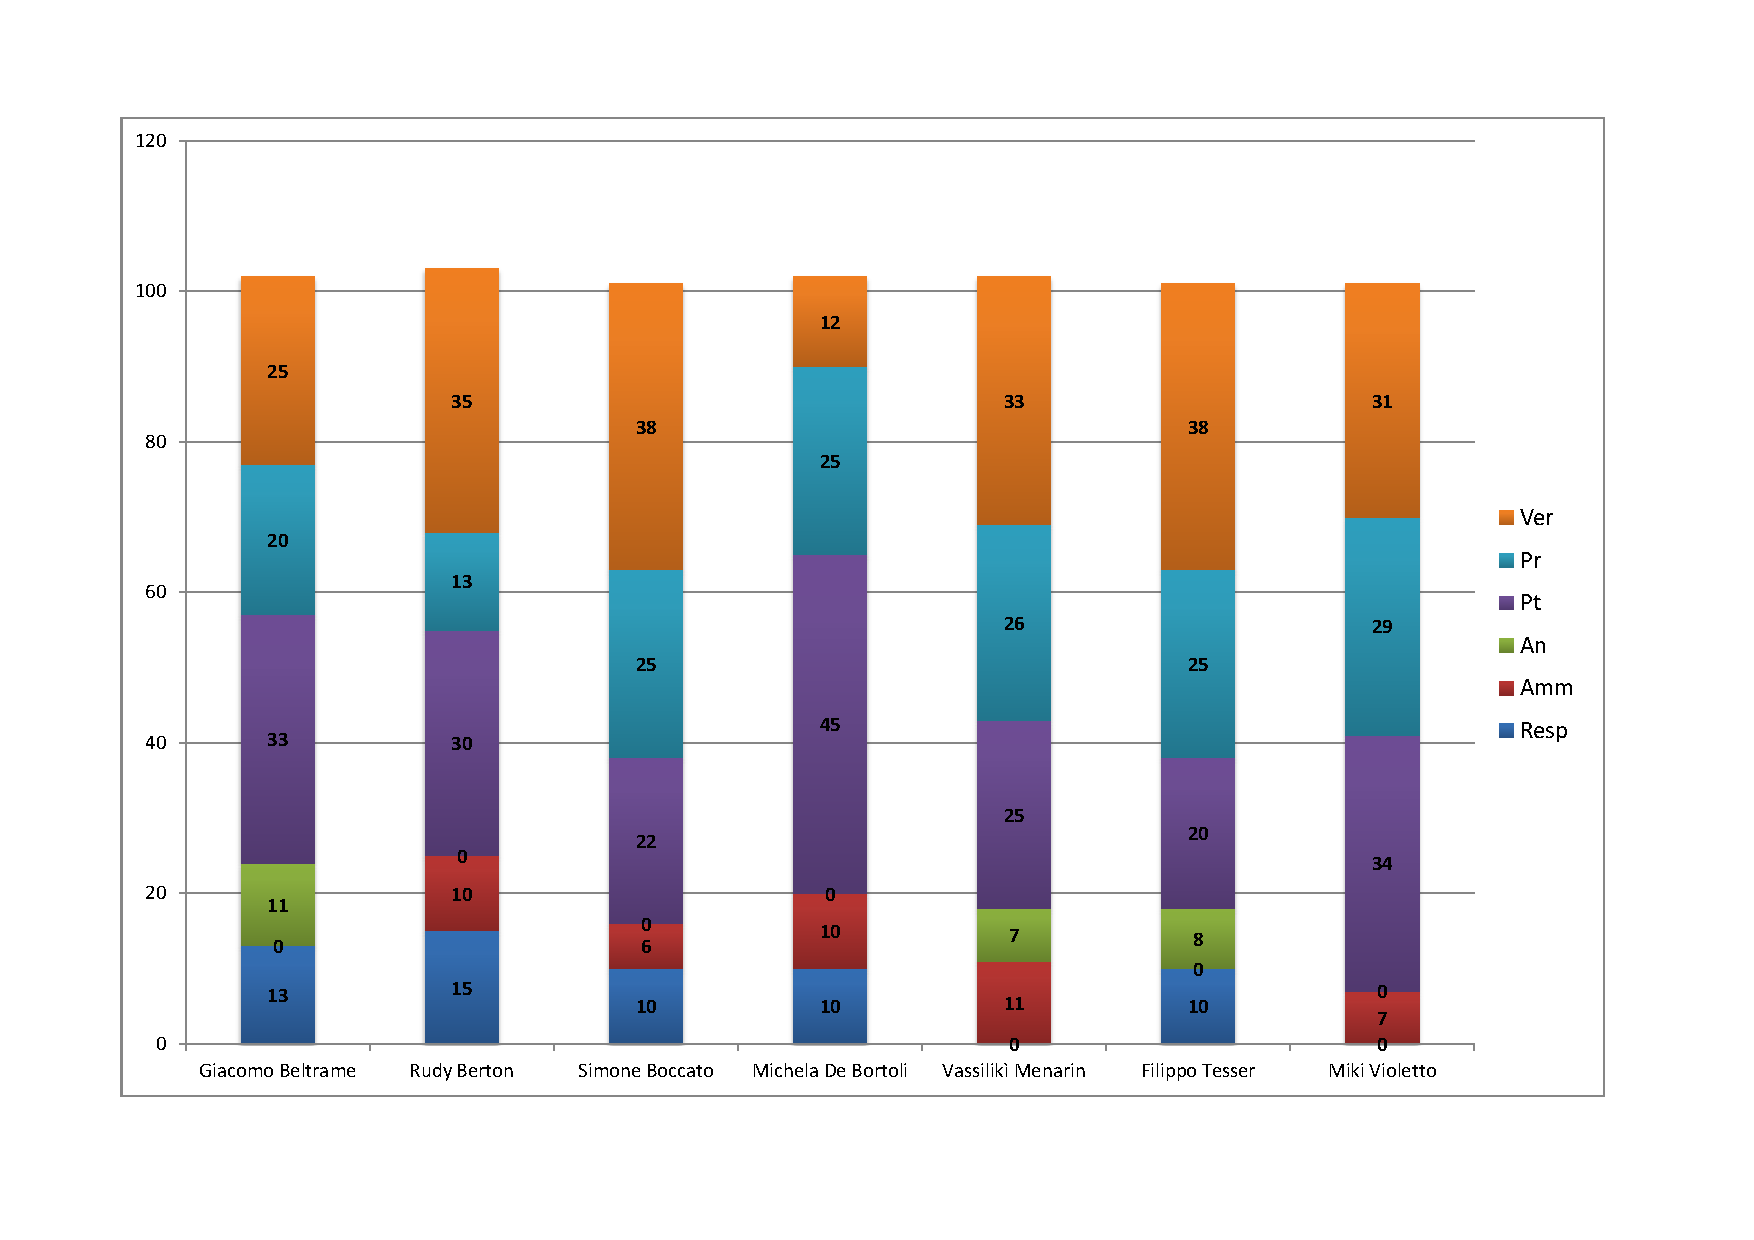
\includegraphics[scale=0.5]{Img/Grafici/Ist07.pdf}
		\caption{ Istogramma: Prospetto orario rendicontato totale}
	\end{figure}
	
	\newpage
	\subsubsection{Prospetto economico}
	Il prospetto economico per le ore rendicontate per ogni ruolo è illustrato in tabella. 
	
	\begin{tabella}{l!{\VRule}c!{\VRule}c}
		
		\color{white} \bold{Ruolo} & \color{white} \bold{Ore} &\color{white} \bold{Spese} \\
		\endfirsthead
		Responsabile & 58 & € 1740 \\
		Amministratore & 44 & € 880\\
		Analista & 26 & € 650 \\
		Progettista & 209 & € 4598 \\
		Programmatore & 163 & € 2445 \\
		Verificatore & 212 & € 3180\\
		Totale & 712 & € 13493\\
		
		\rowcolor{white}  
		\caption{Prospetto economico rendicontato}	    	
		
	\end{tabella}
	
	\begin{figure}[!ht]
		\centering
		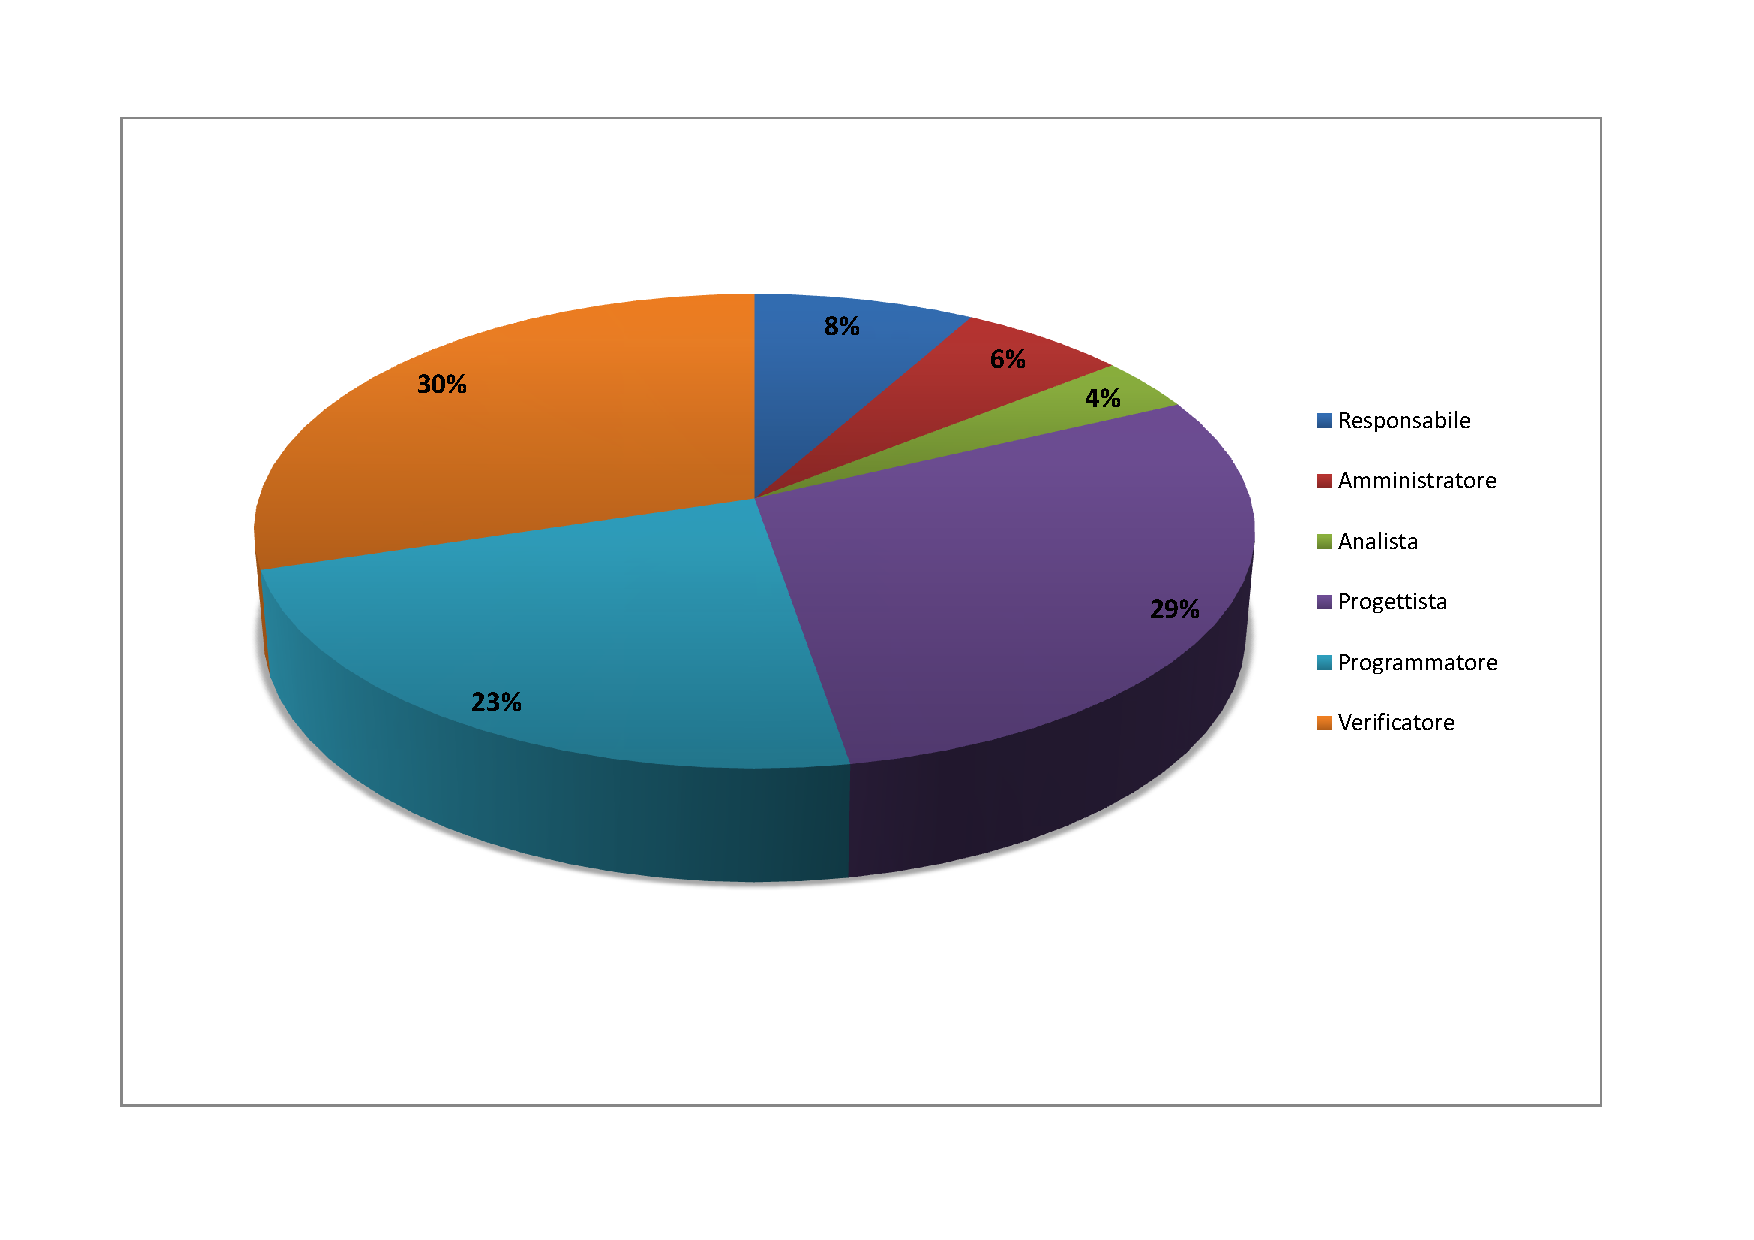
\includegraphics[scale=0.5]{Img/Grafici/Aer07.pdf}
		\caption{ Areogramma: Ore per ruolo rendicontate}
	\end{figure}
	
	\newpage
	\section{Consuntivo e preventivo a finire}
	Eventuali errori di pianificazione rilevati dai consuntivi di periodo sono da imputare a rischi emersi negli stessi. Per un dettaglio dei rischi affrontati vedere l'\hyperref[Attualizzazione dei rischi]{appendice} dedicata.
	\subsection{Attività di progettazione architetturale}
	
	\subsubsection {Consuntivo di periodo}
	Vengono di seguito riportati i costi effettivi sostenuti in questa attività.
	
	\begin{tabella}{l!{\VRule}c!{\VRule}c!{\VRule}c!{\VRule}c!{\VRule}c!{\VRule}c!{\VRule}c}
		
		\color{white} \bold{Nome} & \color{white} \bold{Responsabile} &\color{white} \bold{Amm} & \color{white} \bold{An} & \color{white} \bold{Pt} & \color{white} \bold{Pr} & \color{white} \bold{Ver} & \color{white} \bold{Ore totali persona} \\
		\endfirsthead
		Giacomo Beltrame & 0 & 0 & 5 (+2) & 20 & 0 & 0 & 25 (+2)\\
		Rudy Berton & 0 & 10 (-1) & 0 & 0 & 0 & 13 (-2) & 23 (-3)\\
		Simone Boccato & 0 & 0 & 0 & 5 (+5) & 0 & 20 (-5) & 25\\
		Michela De Bortoli & 10 (-1) & 0 & 0 & 15 (-2) & 0 & 0 & 25 (-3)\\
		Vassilikì Menarin & 0 & 0 & 0 & 15 & 0 & 12 & 27\\
		Filippo Tesser & 10 & 0 & 8 & 0 & 0 & 8 (+2) & 26 (+2)\\
		Miki Violetto & 0 & 7 & 0 & 10 (+2) & 0 & 6 & 23 (+2)\\   
		
		\rowcolor{white}  
		\caption{Consuntivo orario attività di progettazione architetturale}	    	
		
	\end{tabella}	
	
	Segue una tabella che illustra come questi cambiamenti impattino i ruoli e i costi:
	
	
	\begin{tabella}{l!{\VRule}c!{\VRule}c}
		
		\color{white} \bold{Ruolo} & \color{white} \bold{Ore} &\color{white} \bold{Spese} \\
		\endfirsthead
		Responsabile & 20(-1) & € 570 (600-30) \\
		Amministratore & 17(-1) & € 320 (340-20) \\
		Analista & 13(+2) & € 375 (325+50) \\
		Progettista & 65(+5) & € 1540 (1430+110) \\
		Programmatore & 0 & € 0 \\
		Verificatore & 59(-5) & € 810 (885-75)\\
		\hline
		Totale Preventivo & 174  & € 3580\\
		Totale Consuntivo & 174 & € 3615\\
		Differenza & 0 & + € 35\\
		
		\rowcolor{white}  
		\caption{Consuntivo economico attività di progettazione architetturale}	    	
		
	\end{tabella}
	
	\subsubsection{Conclusioni}
	C'è stato un problema protratto di salute di alcuni componenti del \gl{team} che ha portato a una variazione sul carico di ore degli altri componenti per bilanciare, quantificabile con un aumento di budget di €35. 
	
	\subsubsection{Preventivo a finire}
	Durante questa attività c'è stato un errore di pianificazione che ha portato a una spesa non preventivata di €35,00. Considerato che la causa è stata la malattia di diversi membri del gruppo e che si è riusciti comunque a recuperare le ore perse, il gruppo ritiene di non dover modificare la pianificazione futura. Si terrà comunque conto della spesa e si tenterà di farla rientrare nelle fasi successive. Per adesso viene rilevato un bilancio in negativo per una somma pari a \bold{-€35,00}.
	
	\subsection{Attività di progettazione di dettaglio e codifica}
	\subsubsection{Consuntivo di periodo}
	Vengono di seguito riportati i costi effettivi sostenuti in questa attività.
	
	\begin{tabella}{l!{\VRule}c!{\VRule}c!{\VRule}c!{\VRule}c!{\VRule}c!{\VRule}c!{\VRule}c}
		
		\color{white} \bold{Nome} & \color{white} \bold{Responsabile} &\color{white} \bold{Amm} & \color{white} \bold{An} & \color{white} \bold{Pt} & \color{white} \bold{Pr} & \color{white} \bold{Ver} & \color{white} \bold{Ore totali persona} \\
		\endfirsthead
		Giacomo Beltrame & 13 & 0 & 6 & 0 & 20(-1) & 18 & 57 (-1)\\
		Rudy Berton & 0 & 0 & 0 & 30 & 0 & 22 & 52\\
		Simone Boccato & 0 & 6 & 0 & 17 & 25 & 7 & 55\\
		Michela De Bortoli & 0 & 10 & 0 & 20 & 25 & 0 & 55\\
		Vassilikì Menarin & 0 & 0 & 7 & 0 & 26 & 21 (-2) & 54 (-2)\\
		Filippo Tesser & 0 & 0 & 0 & 20 & 15 & 16 & 51\\
		Miki Violetto & 0 & 0 & 0 & 12 (+2) & 29 (-3) & 13 & 54 (-1)\\     
		
		\rowcolor{white}  
		\caption{Consuntivo orario attività di progettazione di dettaglio e codifica}	    	
		
	\end{tabella}	
	
	Segue una tabella che illustra come questi cambiamenti impattino i ruoli e i costi:
	
	
	\begin{tabella}{l!{\VRule}c!{\VRule}c}
		
		\color{white} \bold{Ruolo} & \color{white} \bold{Ore} &\color{white} \bold{Spese} \\
		\endfirsthead
		\endfirsthead
		Responsabile & 13 & € 390 \\
		Amministratore & 16 & € 320\\
		Analista & 13 & € 325 \\
		Progettista & 99(+2) & € 2178 (+44) \\
		Programmatore & 140(-4) & € 2100 (-60) \\
		Verificatore & 97(-2) & € 1455 (-30)\\
		\hline
		Totale Preventivo & 378  & € 6768\\
		Totale Consuntivo & 378 & € 6722\\
		Differenza & 0 & - € 46\\
		
		\rowcolor{white}  
		\caption{Consuntivo economico attività di progettazione di dettaglio e codifica}	    	
		
	\end{tabella}

	\subsubsection{Conclusioni}
	Gli unici problemi da riportare in questa fase sono state delle incongruenze che riguardano alcuni strumenti utilizzati dal \gl{team} e le versioni delle tecnologie da usare, problemi che comunque non hanno portato a ritardi. Il \italics{Responsabile} ha deciso di modificare alcune ore di lavoro per far fronte ad esigenze di organizzazione senza però sforare il totale orario del gruppo. Questa variazione di carico di lavoro ha portato una diminuzione del budget quantificabile con €46.
	
	\subsubsection{Preventivo a finire}
	Durante questa attività ci sono stati dei problemi di entità lieve che riguardano i vari strumenti utilizzati dal gruppo. Questo non ha portato a variazioni sul totale orario e quindi il gruppo non ritiene di dover modificare la pianificazione futura. Il \italics{Responsabile} ha variato il carico di ore per persona portando il bilancio di questa attività in positivo di €46, tenendo conto del bilancio della fase precedente di -€35, il bilancio finale attuale è di -35 + 46 = \bold{+€11}.
	
	\newpage
	\appendix
	\section{Attualizzazione dei rischi} \label{Attualizzazione dei rischi}
	Vengono di seguito indicati i rischi che si sono attualizzati nelle varie attività e come il gruppo li ha superati. Un elenco completo con descrizione dei possibili rischi è presente nella \hyperref[Analisi dei rischi]{sezione 4}.
	
	\subsection{Analisi dei requisiti}
	
	\begin{tabella}{l!{\VRule}>{\centering\arraybackslash}p{6 cm}!{\VRule}>{\centering\arraybackslash}p{3 cm}}
		%{\centering\arraybackslash}p{2 cm}}
		%{l!{\VRule} p{20px} l ! {\VRule}  l !{\VRule}l}
		
		
		\color{white} \bold{Livello} & \color{white} \bold{Tipologia} & \color{white} \bold{Rischio presentatosi} \\
		\endfirsthead
		
		\cellcolor{P} & Scarsa conoscenza delle tecnologie & No \\
		\cellcolor{P} & Guasti \gl{hardware} & No \\
		\multirow{-3}{*}{\cellcolor{P}Tecnologico}	& Malfunzionamenti \gl{software} & No \\
		\hline
		
		\cellcolor{D} & Problemi personali dei membri & \bold{Sì} \\
		\multirow{-2}{*}{\cellcolor{D}Personale} & Problemi interni tra i membri & No \\
		\hline
		
		\cellcolor{P} & Problemi di \gl{versionamento} & \bold{Sì} \\
		\multirow{-2}{*}{\cellcolor{P}Organizzativo} & Errata valutazione dei costi & No \\
		\hline
		
		\rowcolor{D}
		Strumenti & Mancante o insufficiente conoscenza degli strumenti & \bold{Sì} \\	
		\hline	
		
		\rowcolor{P}
		Requisiti & Errata comprensione dei requisiti & \bold{Sì}\\
		\hline
		
		\rowcolor{white}  
		\caption{Attualizzazione dei rischi nell'attività di analisi dei requisiti}	    	
		
	\end{tabella}
	
	\subsubsection{Problemi personali dei membri}
	I membri del gruppo hanno avuto dei problemi famigliari mentre altri sono stati impossibilitati a lavorare per malattia. La pianificazione ha permesso di rispettare comunque le scadenze; i membri hanno tempestivamente informato il responsabile e, quando malati, il carico di lavoro è stato ripartito per non rallentare troppo i lavori.
	
	\subsubsection{Problemi di versionamento}
	I membri hanno avuto dei problemi a individuare la corretta versione dei documenti, soprattutto quando questi erano modificati da più persone. Il problema è stato più spiccato all'inizio, prima che il gruppo prendesse dimestichezza con \gl{tracker}, ed è stato definitivamente risolto appena i membri hanno imparato a usarlo correttamente.
	
	\subsubsection{Mancante o insufficiente conoscenza degli strumenti}
	Come specificato nella sottosezione recedente, i membri hanno avuto una difficoltà iniziale ad usare \gl{tracker}. Questo problema, di cui si era comunque tenuto conto, è stato risolto nelle fasi iniziali grazie agli amministratori, che hanno fornito precise istruzioni e regole per il corretto utilizzo dello strumento in questione.
	
	\subsubsection{Errata comprensione dei requisiti}
	Dopo la presentazione del capitolato in aula e in seguito a un primo incontro con il committente, il gruppo ha cominciato a lavorare alla raccolta dei requisiti. Sono emerse delle incomprensioni e dei dubbi sulla correttezza dei requisiti individuati. Avendo programmato un secondo incontro col committente, questi problemi sono stati chiariti e, sul totale, si è rilevato un leggero ritardo nella stesura dell'\doc{Analisi dei requisiti}, comunque compensata dalla fase di \gl{slack} predisposta.
	
	\subsection{Raffinamento dei requisiti}
	
	\begin{tabella}{l!{\VRule}>{\centering\arraybackslash}p{6 cm}!{\VRule}>{\centering\arraybackslash}p{3 cm}}
		%{\centering\arraybackslash}p{2 cm}}
		%{l!{\VRule} p{20px} l ! {\VRule}  l !{\VRule}l}
		
		
		\color{white} \bold{Livello} & \color{white} \bold{Tipologia} & \color{white} \bold{Rischio presentatosi} \\
		\endfirsthead
		
		\cellcolor{P} & Scarsa conoscenza delle tecnologie & No \\
		\cellcolor{P} & Guasti \gl{hardware} & No \\
		\multirow{-3}{*}{\cellcolor{P}Tecnologico}	& Malfunzionamenti \gl{software} & No \\
		\hline
		
		\cellcolor{D} & Problemi personali dei membri & No \\
		\multirow{-2}{*}{\cellcolor{D}Personale} & Problemi interni tra i membri & No \\
		\hline
		
		\cellcolor{P} & Problemi di \gl{versionamento} & No \\
		\multirow{-2}{*}{\cellcolor{P}Organizzativo} & Errata valutazione dei costi & No \\
		\hline
		
		\rowcolor{D}
		Strumenti & Mancante o insufficiente conoscenza degli strumenti & No \\	
		\hline	
		
		\rowcolor{P}
		Requisiti & Errata comprensione dei requisiti & No\\
		\hline
		
		\rowcolor{white}  
		\caption{Attualizzazione dei rischi nell'attività di progettazione architetturale}	    	
		
	\end{tabella}
	
	Data la breve durata dell'attività e la sua semplicità non si sono presentati problemi.
	
	\subsection{Progettazione architetturale}
	
	\begin{tabella}{l!{\VRule}>{\centering\arraybackslash}p{6 cm}!{\VRule}>{\centering\arraybackslash}p{3 cm}}
		%{\centering\arraybackslash}p{2 cm}}
		%{l!{\VRule} p{20px} l ! {\VRule}  l !{\VRule}l}
		
		
		\color{white} \bold{Livello} & \color{white} \bold{Tipologia} & \color{white} \bold{Rischio presentatosi} \\
		\endfirsthead
		
		\cellcolor{P} & Scarsa conoscenza delle tecnologie & No \\
		\cellcolor{P} & Guasti \gl{hardware} & No \\
		\multirow{-3}{*}{\cellcolor{P}Tecnologico}	& Malfunzionamenti \gl{software} & No \\
		\hline
		
		\cellcolor{D} & Problemi personali dei membri & \bold{Sì} \\
		\multirow{-2}{*}{\cellcolor{D}Personale} & Problemi interni tra i membri & No \\
		\hline
		
		\cellcolor{P} & Problemi di \gl{versionamento} & No \\
		\multirow{-2}{*}{\cellcolor{P}Organizzativo} & Errata valutazione dei costi & No \\
		\hline
		
		\rowcolor{D}
		Strumenti & Mancante o insufficiente conoscenza degli strumenti & \bold{Sì} \\	
		\hline	
		
		\rowcolor{P}
		Requisiti & Errata comprensione dei requisiti & No\\
		\hline
		
		\rowcolor{white}  
		\caption{Attualizzazione dei rischi nell'attività di progettazione architetturale}	    	
		
	\end{tabella}
	
	\subsubsection{Problemi personali dei membri}
	Due membri del gruppo sono stati impossibilitati a lavorare per problemi di salute. La pianificazione ha permesso di rispettare comunque le scadenze, i membri hanno tempestivamente informato il responsabile che ha ridistribuito il carico di ore per rimanere dentro le scadenze. Ciò ha permesso di finire il lavoro ma il ritardo accumulato ha portato ad una mancata riunione con il proponente.
	
	\subsubsection{Mancante o insufficiente conoscenza degli strumenti}
	Nelle prime fasi di progettazione sono sorti problemi per la scarsa conoscenza con \gl{StarUML} per quanto riguarda la creazione dei diagrammi di attività e \gl{package}. I problemi sono stati risolti nel tempo tramite lettura di guide dedicate da parte dei \italics{Progettisti}.
	
	\subsection{Progettazione di dettaglio e codifica}
	
	\begin{tabella}{l!{\VRule}>{\centering\arraybackslash}p{6 cm}!{\VRule}>{\centering\arraybackslash}p{3 cm}}
		%{\centering\arraybackslash}p{2 cm}}
		%{l!{\VRule} p{20px} l ! {\VRule}  l !{\VRule}l}
		
		
		\color{white} \bold{Livello} & \color{white} \bold{Tipologia} & \color{white} \bold{Rischio presentatosi} \\
		\endfirsthead
		
		\cellcolor{P} & Scarsa conoscenza delle tecnologie & No \\
		\cellcolor{P} & Guasti \gl{hardware} & No \\
		\multirow{-3}{*}{\cellcolor{P}Tecnologico}	& Malfunzionamenti \gl{software} & \bold{Sì} \\
		\hline
		
		\cellcolor{D} & Problemi personali dei membri & No \\
		\multirow{-2}{*}{\cellcolor{D}Personale} & Problemi interni tra i membri & No \\
		\hline
		
		\cellcolor{P} & Problemi di \gl{versionamento} & No \\
		\multirow{-2}{*}{\cellcolor{P}Organizzativo} & Errata valutazione dei costi & No \\
		\hline
		
		\rowcolor{D}
		Strumenti & Mancante o insufficiente conoscenza degli strumenti & \bold{Sì} \\	
		\hline	
		
		\rowcolor{P}
		Requisiti & Errata comprensione dei requisiti & No\\
		\hline
		
		\rowcolor{white}  
		\caption{Attualizzazione dei rischi nell'attività di progettazione di dettaglio e codifica}	    	
		
	\end{tabella}
	
	\subsubsection{Malfunzionamenti software}
	Si sono presentate delle incongruenze tra le varie versioni delle tecnologie scelte. Nel caso più grave questo ha portato alla riscrittura di alcune parti di codice a causa dell'utilizzo di metodi divenuti obsoleti nelle versioni scelte e che rendevano il funzionamento del prodotto instabile. L'\italics{Amministratore} ha provveduto tempestivamente a fare aggiornare i \gl{software} dei membri coinvolti. La celerità di questa azione non ha portato a ritardi.
	
	\subsubsection{Mancante o insufficiente conoscenza degli strumenti}
	Alcuni membri non erano a conoscenza dei meccanismi di automatizzazione offerti dall'\gl{IDE} scelto per la codifica.
	L'\italics{Amministratore} ha provveduto a configurare ed illustrare tali meccanismi ai membri interessati. La risoluzione tempestiva di questo problema non ha portato ulteriori ritardi.
		
	\newpage
	\section{Attività di investimento} \label{Investimento}
	Le attività di Analisi dei requisiti utente e di Raffinamento dei requisiti non sono a carico del committente e rappresentano l'investimento iniziale del gruppo. Si è scelto di riscrivere comunque, in questa appendice, i prospetti economici e orari delle fasi in questione per completezza e offrire al committente maggiori informazioni sull'operato del gruppo. Per il preventivo delle fasi rendicontate si veda la \hyperref[Preventivo] {Sezione 6}.
	
	
	\subsection{Analisi dei requisiti utente}
	\subsubsection{Prospetto orario}
	Durante questa prima attività ogni componente del gruppo ricoprirà i seguenti ruoli:
	
	\begin{tabella}{l!{\VRule}c!{\VRule}c!{\VRule}c!{\VRule}c!{\VRule}c!{\VRule}c!{\VRule}c!{\VRule}c}
		
		\color{white} \bold{Nome} & \color{white} \bold{Responsabile} &\color{white} \bold{Amm} & \color{white} \bold{An} & \color{white} \bold{Pt} & \color{white} \bold{Pr} & \color{white} \bold{Ver} & \color{white} \bold{Ore totali persona} \\
		\endfirsthead
		Giacomo Beltrame & 0 & 22 & 0 & 0 & 0 & 10 & 32\\
		Rudy Berton & 0 & 0 & 20 & 0 & 0 & 10 & 30\\
		Simone Boccato & 0 & 0 & 30 & 0 & 0 & 8 & 38\\
		Michela De Bortoli & 0 & 0 & 26 & 0 & 0 & 12 & 38\\
		Vassilikì Menarin & 20 & 0 & 0 & 0 & 0 & 15 & 35\\
		Filippo Tesser & 0 & 17 & 0 & 0 & 0 & 18 & 35\\
		Miki Violetto & 0 & 0 & 26 & 0 & 0 & 10 & 36\\   
		
		\rowcolor{white}  
		\caption{Prospetto orario attività di analisi}	    	
		
	\end{tabella}
	\newpage
	\begin{figure}[!ht]
		\centering
		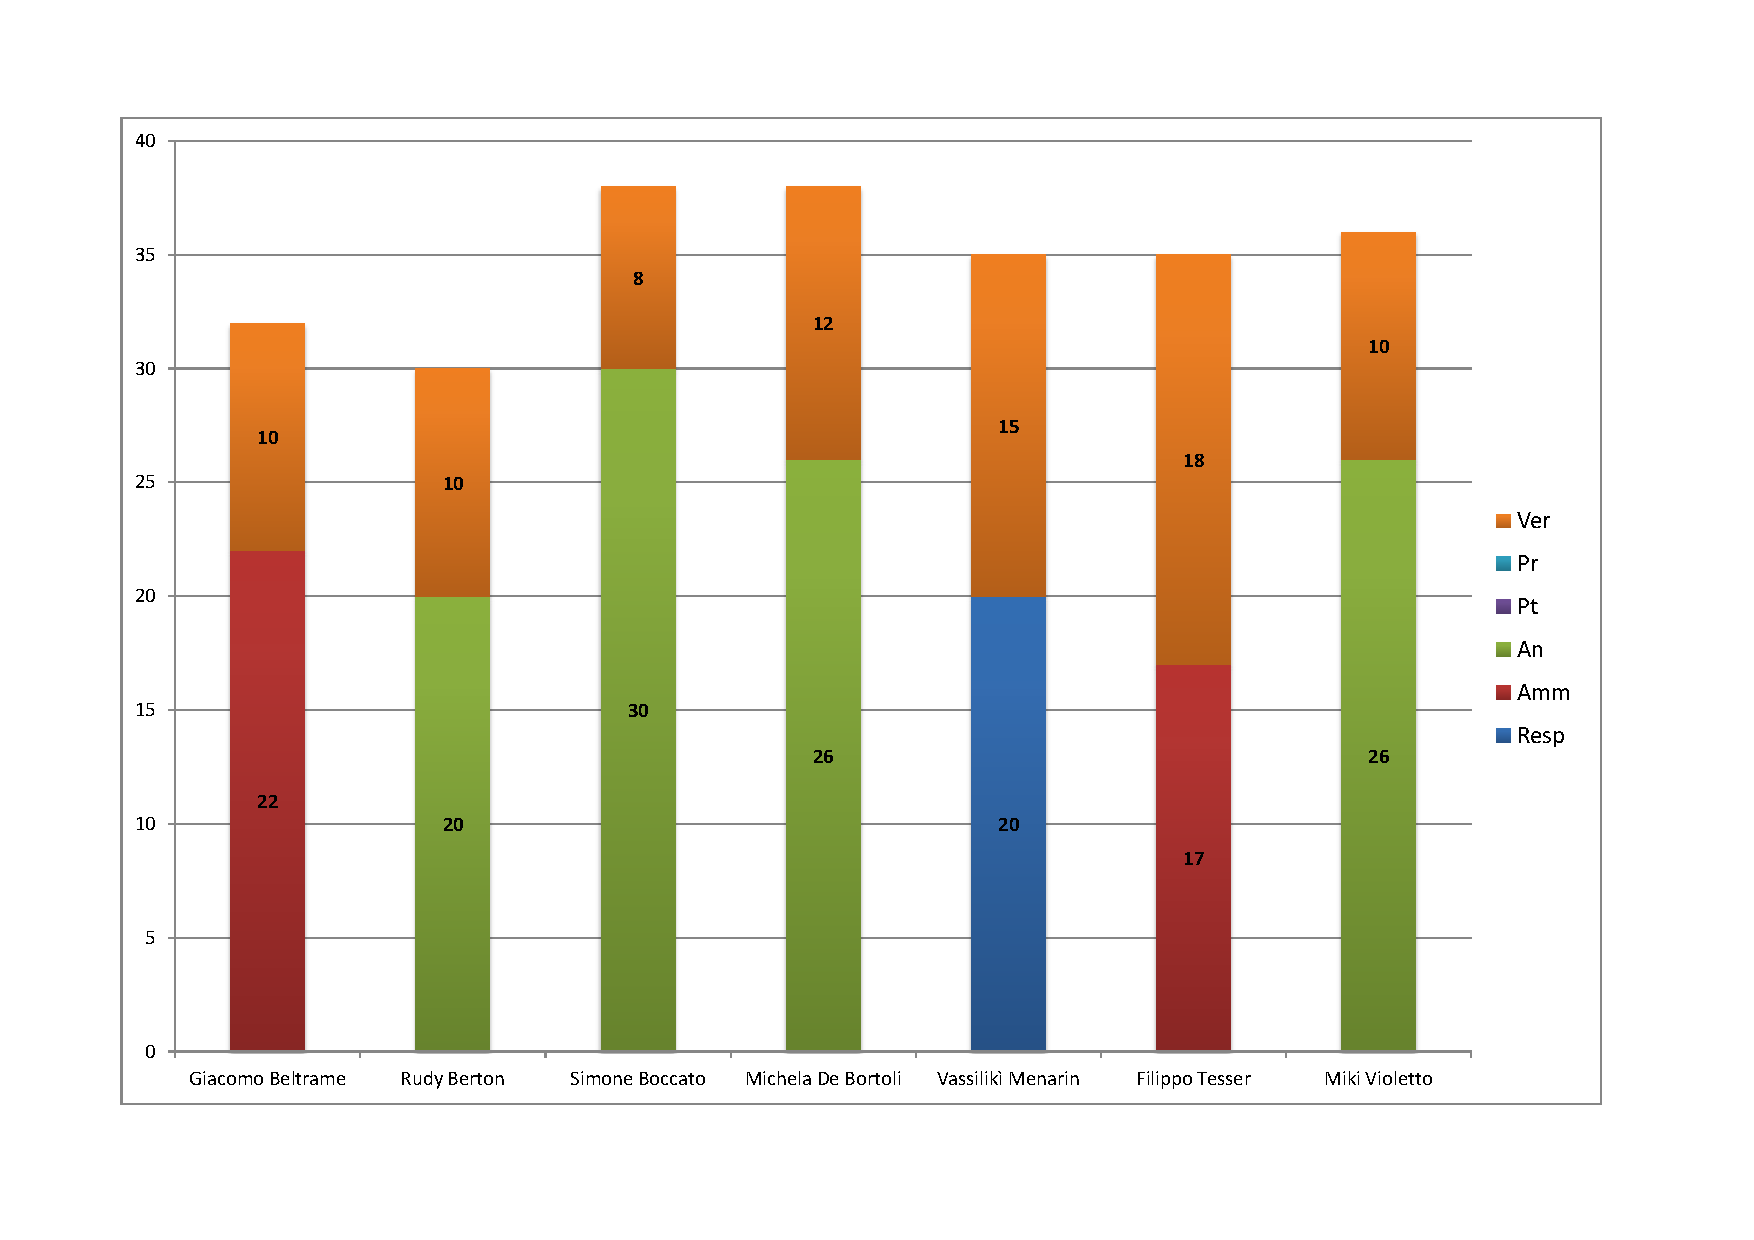
\includegraphics[scale=0.5]{Img/Grafici/Ist01.pdf}
		\caption{ Istogramma: Prospetto orario attività di analisi}
	\end{figure}
	
	\newpage
	\subsubsection{Prospetto economico}
	Il prospetto economico per questa attività è illustrato in tabella. Notare che le spese per questa attività \bold{non} sono a carico del proponente.
	
	\begin{tabella}{l!{\VRule}c!{\VRule}c}
		
		\color{white} \bold{Ruolo} & \color{white} \bold{Ore} &\color{white} \bold{Spese} \\
		\endfirsthead
		Responsabile & 20 & € 600 \\
		Amministratore & 39 & € 780 \\
		Analista & 102 & € 2550 \\
		Progettista & 0 & € 0 \\
		Programmatore & 0 & € 0 \\
		Verificatore & 83 & € 1245 \\
		Totale & 244  & € 5175\\
		
		\rowcolor{white}  
		\caption{Prospetto economico attività di analisi}	    	
		
	\end{tabella}
	
	\begin{figure}[!ht]
		\centering
		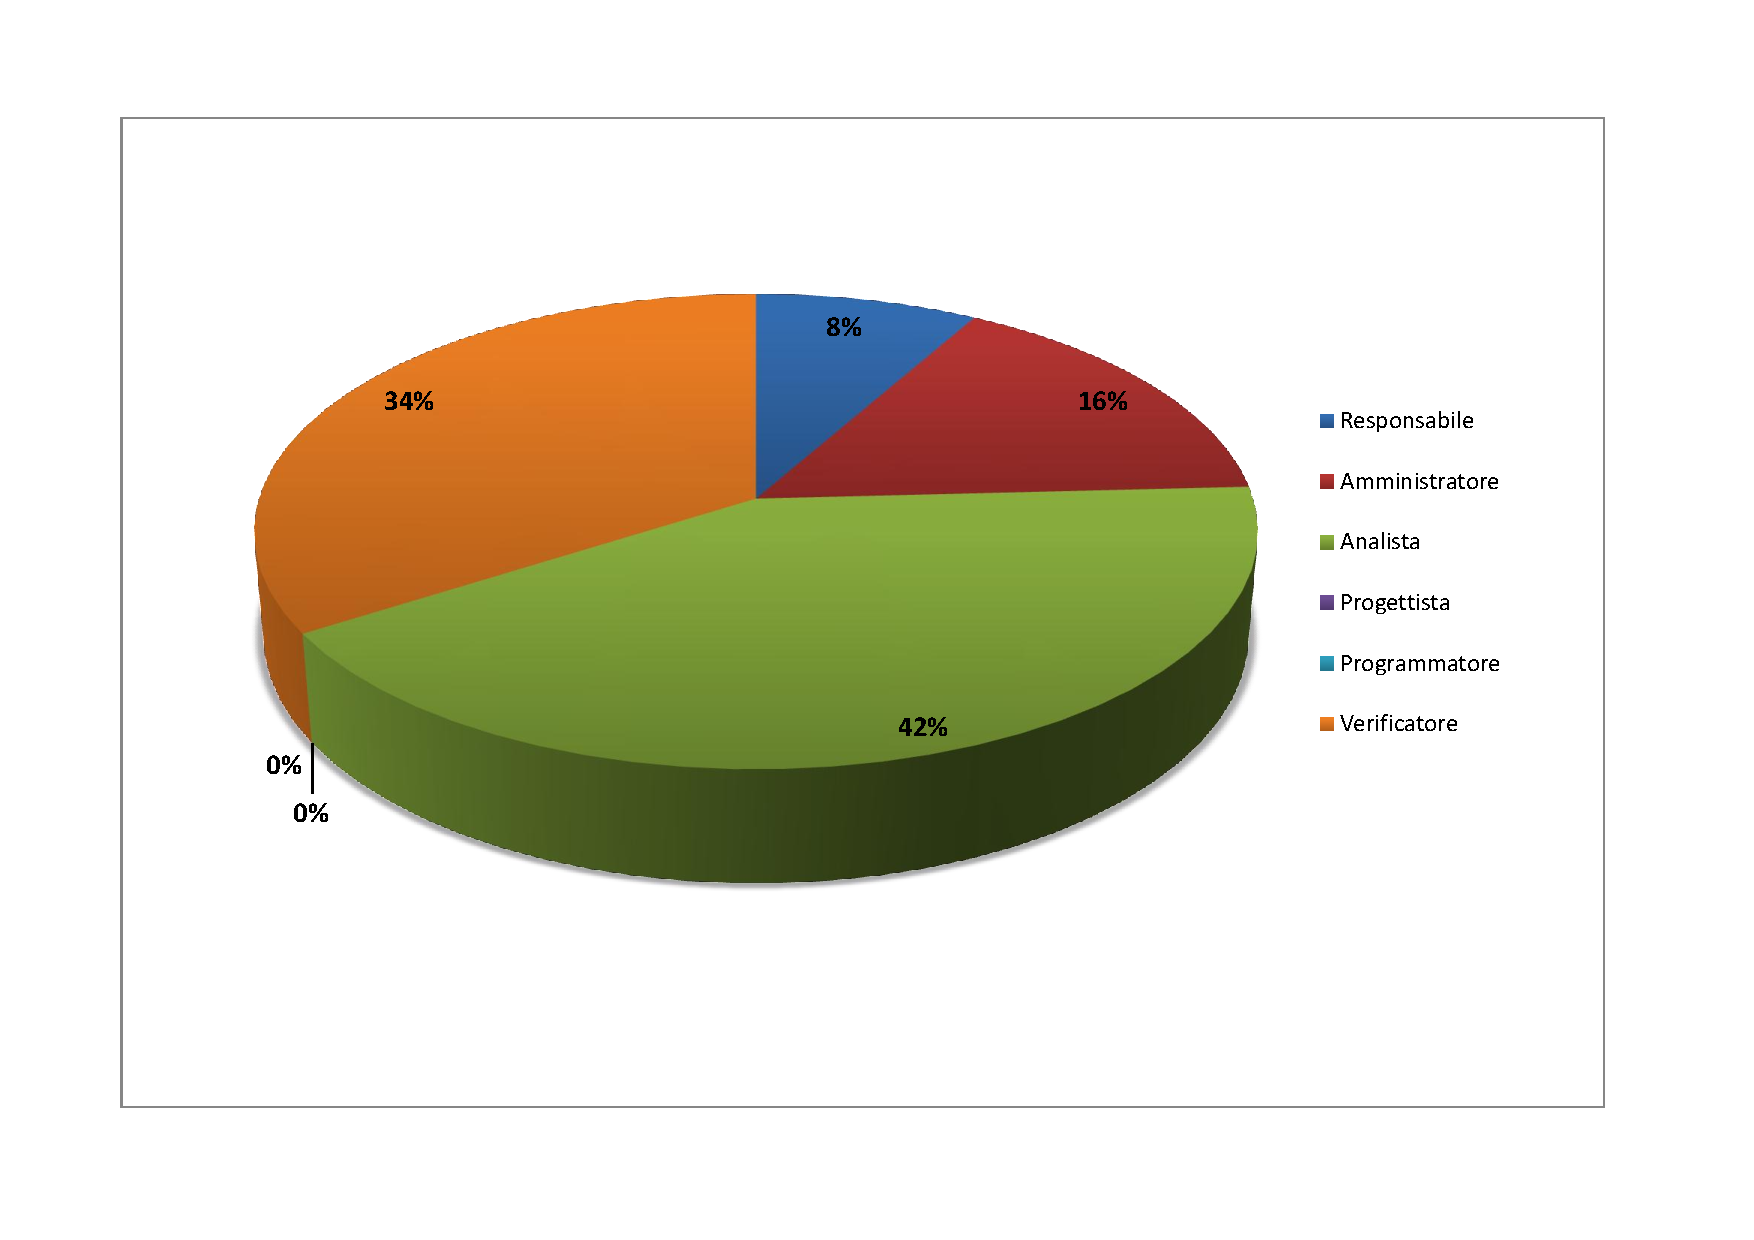
\includegraphics[scale=0.5]{Img/Grafici/Aer01.pdf}
		\caption{ Areogramma: Ore per ruolo durante l'attività di analisi}
	\end{figure}
	
	\subsubsection{Consuntivo}
	Vengono di seguito riportati i costi effettivi sostenuti in questa attività. Si ricorda che questa tabella vuole fornire informazioni sul modo di procedere del gruppo e sulla sua capacità di rispettare la pianificazione, perché questa attività non è a carico del committente.
	
	\begin{tabella}{l!{\VRule}c!{\VRule}c!{\VRule}c!{\VRule}c!{\VRule}c!{\VRule}c!{\VRule}c!{\VRule}c}
		
		\color{white} \bold{Nome} & \color{white} \bold{Responsabile} &\color{white} \bold{Amm} & \color{white} \bold{An} & \color{white} \bold{Pt} & \color{white} \bold{Pr} & \color{white} \bold{Ver} & \color{white} \bold{Ore totali persona} \\
		\endfirsthead
		Giacomo Beltrame & 0 & 22 & 0 & 0 & 0 & 10 (+2) & 32(+2)\\
		Rudy Berton & 0 & 0 & 20 (+2) & 0 & 0 & 10 & 30(+2)\\
		Simone Boccato & 0 & 0 & 30 & 0 & 0 & 8 & 38\\
		Michela De Bortoli & 0 & 0 & 26 & 0 & 0 & 12(-2) & 38 (-2)\\
		Vassilikì Menarin & 20 & 0 & 0 & 0 & 0 & 15 (+2) & 35(+2)\\
		Filippo Tesser & 0 & 17(+3) & 0 & 0 & 0 & 18 & 35(+3)\\
		Miki Violetto & 0 & 0 & 26 (-3)& 0 & 0 & 10 & 36(-3)\\   
		
		\rowcolor{white}  
		\caption{Consuntivo orario attività di analisi}	    	
		
	\end{tabella}
	
	Segue una tabella che illustra come questi cambiamenti impattino i ruoli e i costi:
	
	\begin{tabella}{l!{\VRule}c!{\VRule}c}
		
		\color{white} \bold{Ruolo} & \color{white} \bold{Ore} &\color{white} \bold{Spese} \\
		\endfirsthead
		Responsabile & 20 & € 600 \\
		Amministratore & 39(+3) & € 840 (780+60) \\
		Analista & 102(-1) & € 2525 (2550-25) \\
		Progettista & 0 & € 0 \\
		Programmatore & 0 & € 0 \\
		Verificatore & 83(+2) & € 1275 (1245+30)\\
		\hline
		Totale Preventivo & 244  & € 5175\\
		Totale Consuntivo & 249 & € 5280\\
		Differenza & +5 & + € 65\\
		
		\rowcolor{white}  
		\caption{Consuntivo economico attività di analisi}	    	
		
	\end{tabella}
	
	\subsubsection{Conclusioni}
	C'è stato un errore di pianificazione che ha portato a un'incremento di 5 ore, quantificabili con un aumento di budget di €65. Considerato che l'errore maggiore, sia in termini orari, sia economici, è stato fatto per il ruolo di amministratore, il gruppo ritiene di non dover modificare la pianificazione futura. Infatti, questo incremento è dovuto all'impegno aggiuntivo che l'amministratore ha dovuto porre nella messa a punto e nella spiegazione del sistema di tracking.
	
	\newpage
	\subsection{Raffinamento dei requisiti}
	\subsubsection{Prospetto orario}
	Durante questa attività ogni componente del gruppo ricoprirà i seguenti ruoli:
	
	\begin{tabella}{l!{\VRule}c!{\VRule}c!{\VRule}c!{\VRule}c!{\VRule}c!{\VRule}c!{\VRule}c!{\VRule}c}
		
		\color{white} \bold{Nome} & \color{white} \bold{Responsabile} &\color{white} \bold{Amm} & \color{white} \bold{An} & \color{white} \bold{Pt} & \color{white} \bold{Pr} & \color{white} \bold{Ver} & \color{white} \bold{Ore totali persona} \\
		\endfirsthead
		Giacomo Beltrame & 0 & 0 & 4 & 0 & 0 & 7 & 11\\
		Rudy Berton & 0 & 7 & 0 & 0 & 0 & 6 & 13\\
		Simone Boccato & 0 & 6 & 0 & 0 & 0 & 5 & 11\\
		Michela De Bortoli & 0 & 0 & 0 & 0 & 0 & 10 & 10\\
		Vassilikì Menarin & 0 & 0 & 7 & 0 & 0 & 5 & 12\\
		Filippo Tesser & 0 & 0 & 4 & 0 & 0 & 7 & 11\\
		Miki Violetto & 12 & 3 & 0 & 0 & 0 & 3 & 18\\   
		
		\rowcolor{white}  
		\caption{Prospetto orario attività di raffinamento dei requisiti}	    	
		
	\end{tabella}
	
	\begin{figure}[!ht]
		\centering
		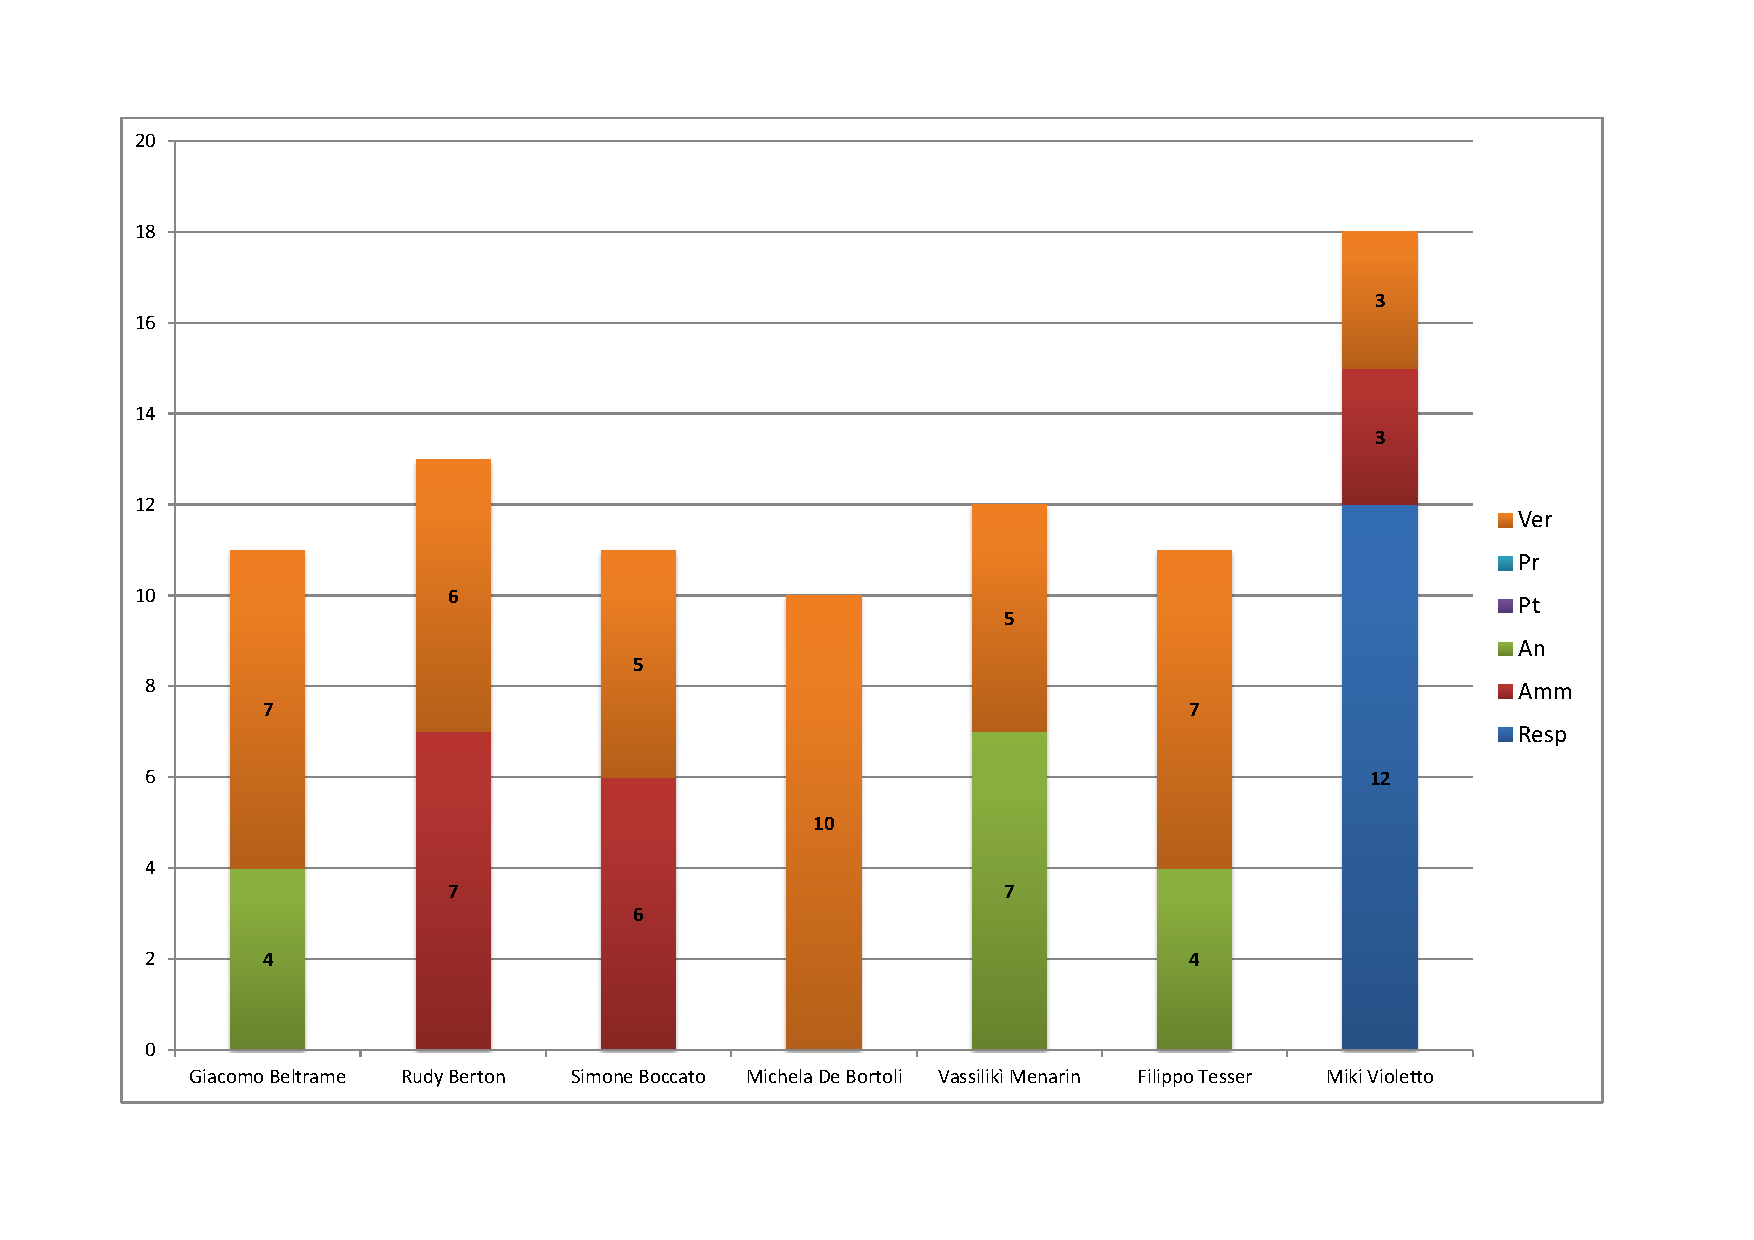
\includegraphics[scale=0.5]{Img/Grafici/Ist02.pdf}
		\caption{ Istogramma: Prospetto orario attività di raffinamento dei requisiti}
	\end{figure}
	
	\newpage
	\subsubsection{Prospetto economico}
	Il prospetto economico per questa attività è illustrato in tabella. Notare che le spese per questa attività \bold{non} sono a carico del proponente.
	
	\begin{tabella}{l!{\VRule}c!{\VRule}c}
		
		\color{white} \bold{Ruolo} & \color{white} \bold{Ore} &\color{white} \bold{Spese} \\
		\endfirsthead
		Responsabile & 12 & € 360 \\
		Amministratore & 16 & € 320\\
		Analista & 15 & € 375 \\
		Progettista & 0 & € 0 \\
		Programmatore & 0 & € 0 \\
		Verificatore & 43 & € 645 \\
		Totale & 86  & € 1700\\
		
		\rowcolor{white}  
		\caption{Prospetto economico attività di raffinamento dei requisiti}	    	
		
	\end{tabella}
	
	\begin{figure}[!ht]
		\centering
		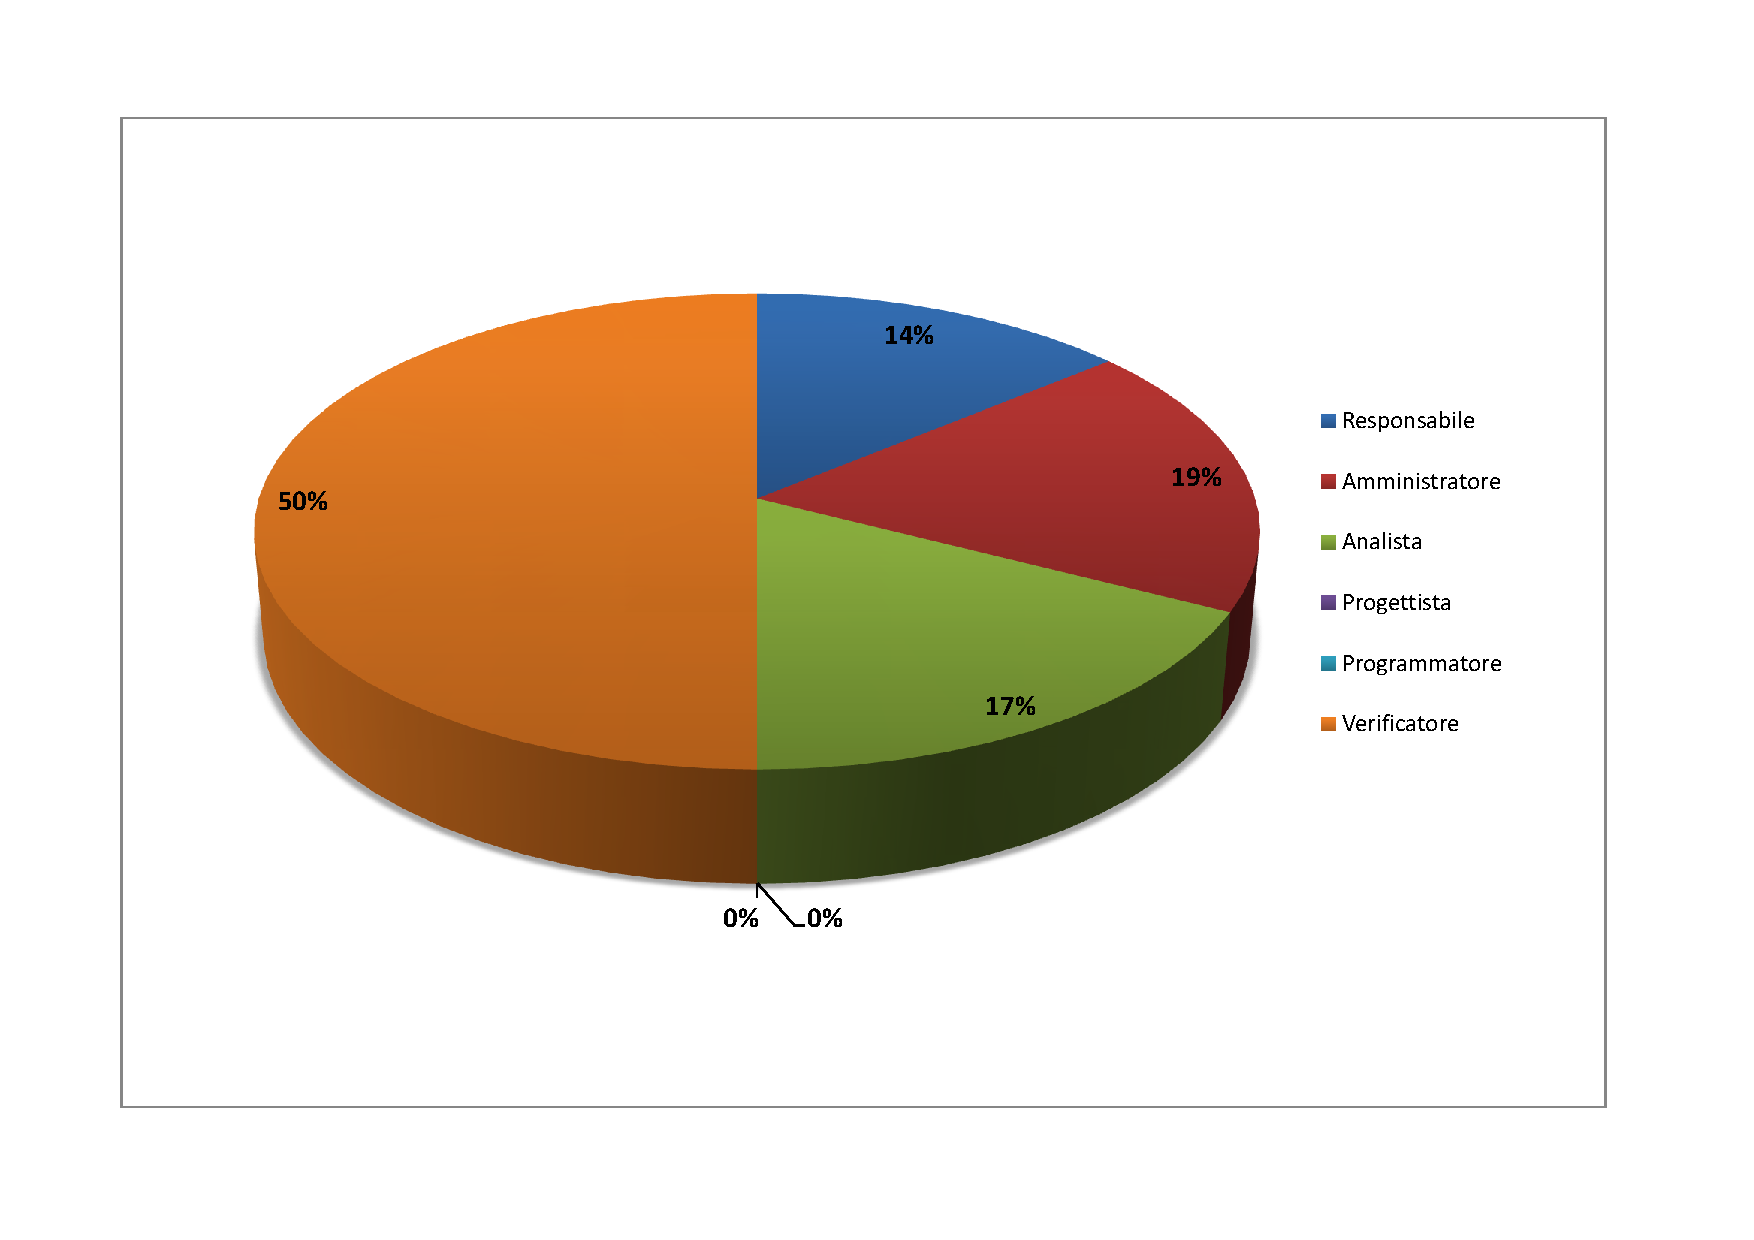
\includegraphics[scale=0.5]{Img/Grafici/Aer02.pdf}
		\caption{ Areogramma: Ore per ruolo durante l'attività di raffinamento dei requisiti}
	\end{figure}
	
	\subsubsection{Consuntivo}
	Vengono di seguito riportati i costi effettivi sostenuti in questa attività. Si ricorda che questa tabella vuole fornire informazioni sul modo di procedere del gruppo e sulla sua capacità di rispettare la pianificazione, perché questa attività non è a carico del committente.
	
	\begin{tabella}{l!{\VRule}c!{\VRule}c!{\VRule}c!{\VRule}c!{\VRule}c!{\VRule}c!{\VRule}c!{\VRule}c}
	
		\color{white} \bold{Nome} & \color{white} \bold{Responsabile} &\color{white} \bold{Amm} & \color{white} \bold{An} & \color{white} \bold{Pt} & \color{white} \bold{Pr} & \color{white} \bold{Ver} & \color{white} \bold{Ore totali persona} \\
		\endfirsthead
		Giacomo Beltrame & 0 & 0 & 4 & 0 & 0 & 7 & 11\\
		Rudy Berton & 0 & 7 & 0 & 0 & 0 & 6 & 13\\
		Simone Boccato & 0 & 6 & 0 & 0 & 0 & 5 & 11\\
		Michela De Bortoli & 0 & 0 & 0 & 0 & 0 & 10 & 10\\
		Vassilikì Menarin & 0 & 0 & 7 & 0 & 0 & 5 & 12\\
		Filippo Tesser & 0 & 0 & 4 & 0 & 0 & 7 & 11\\
		Miki Violetto & 12 & 3 & 0 & 0 & 0 & 3 & 18\\     
			
		\rowcolor{white}  
		\caption{Consuntivo orario attività di analisi}	    	
			
	\end{tabella}
			
	Segue una tabella che illustra come questi cambiamenti impattino i ruoli e i costi:
			
	\begin{tabella}{l!{\VRule}c!{\VRule}c}
				
		\color{white} \bold{Ruolo} & \color{white} \bold{Ore} &\color{white} \bold{Spese} \\
		\endfirsthead
		Responsabile & 12 & € 360 \\
		Amministratore & 16 & € 320\\
		Analista & 15 & € 375 \\
		Progettista & 0 & € 0 \\
		Programmatore & 0 & € 0 \\
		Verificatore & 43 & € 645 \\
		Totale & 86  & € 1700\\
		
		\rowcolor{white}  
		\caption{Consuntivo economico attività di analisi}	    	
				
	\end{tabella}
	
	\subsubsection{Conclusioni}
	Il gruppo ha rispettato la pianificazione e questa attività non ha avuto imprevisti.
	
	\newpage
	\section{Organigramma}
	
	\subsection{Redazione}
	
	\begin{tabella}{l!{\VRule}c!{\VRule}c}
		
		\color{white} \bold{Nominativo} & \color{white} \bold{Data} &\color{white} \bold{Firma} \\
		\endfirsthead
		
		Vassilikì Menarin & 14.01.2016 & 
\includegraphics[scale=0.15]{Img/Firme/Viki.png} \\
		
	\end{tabella}
	
	\subsection{Approvazione}
	
	\begin{tabella}{l!{\VRule}c!{\VRule}c}
		
		\color{white} \bold{Nominativo} & \color{white} \bold{Data} &\color{white} \bold{Firma} \\
		\endfirsthead
		
		Vassilikì Menarin & 17.01.2016 & 
\includegraphics[scale=0.15]{Img/Firme/Viki.png} \\
		Tullio Vardanega &  &  \\  		
		
	\end{tabella}
	
	\subsection{Accettazione dei componenti}
	
	\begin{tabella}{l!{\VRule}c!{\VRule}c}
		
		\color{white} \bold{Nominativo} & \color{white} \bold{Data di accettazione} &\color{white} \bold{Firma} \\
		\endfirsthead
		
		Giacomo Beltrame & 18.12.2015 & 
\includegraphics[scale=0.15]{Img/Firme/Giacomo.png} \\
		Rudy Berton & 18.12.2015 & 
\includegraphics[scale=0.15]{Img/Firme/Rudy.png} \\
		Simone Boccato & 18.12.2015 & 
\includegraphics[scale=0.15]{Img/Firme/Simone.png} \\
		Michela De Bortoli & 18.12.2015 & 
\includegraphics[scale=0.15]{Img/Firme/Michela.png} \\
		Vassilikì Menarin & 18.12.2015 & 
\includegraphics[scale=0.15]{Img/Firme/Viki.png} \\
		Filippo Tesser& 18.12.2015 & 
\includegraphics[scale=0.15]{Img/Firme/Filippo.png} \\
		Miki Violetto & 18.12.2015 & 
\includegraphics[scale=0.15]{Img/Firme/Miki.png} \\	 		
		
	\end{tabella}
	
	\subsection{Componenti}
	
	\begin{tabella}{l!{\VRule}c!{\VRule}c}
		
		\color{white} \bold{Nominativo} & \color{white} \bold{Matricola} &\color{white} \bold{Indirizzo e-mail} \\
		\endfirsthead
		
		Giacomo Beltrame & 1006153 & giacomo.beltrame.91@gmail.com \\
		Rudy Berton & 1049443 & rudyberton92@gmail.com \\
		Simone Boccato & 1047882 & boccato92@gmail.com \\
		Michela De Bortoli & 1027000 & shirun9215@gmail.com\\
		Vassilikì Menarin & 1049663 & vassiliki.menarin@gmail.com \\	Filippo Tesser& 1009236 & filippo90t@gmail.com \\
		Miki Violetto & 1029140 & mikiww2@gmail.com\\	 		
		
	\end{tabella}
	
	\subsection{Note}
	I ruoli sono stati ripartiti come visibile nelle tabelle presenti nella sezione \hyperref[Preventivo]{Preventivo}. Si è fatto in modo che tutti i membri del gruppo ricoprissero tutti i ruoli e che i verificatori non verificassero mai le attività svolte da loro stessi.
	
	
\end{document}
